\documentclass[mathserif]{beamer}
\usepackage[sc]{mathpazo}
\usepackage[utf8]{inputenc}
%\usepackage{lmodern}
\usepackage{amsfonts}
\usepackage{graphicx}
\usepackage{color}
%\usepackage{mathtools}
\newtheorem{ineq}{Inequality}
\newtheorem{eq}{Equality}
\newtheorem{target}{Target}
\newtheorem{obs}{Observation}
\newtheorem{pty}{Property}
\usetheme{Berlin}
\useoutertheme{infolines}
\setbeamertemplate{navigation symbols}{}
%\setbeamertemplate{theorems}[numbered]
\title[Stochastic Process]{Lecture notes of Stochastic Process}
\subtitle{lectured by prof. Hsueh-I Lu}
\author{pishen}
\institute[AlgoLab]{AlgoLab, CSIE, NTU}

\begin{document}
\begin{frame}[plain]
	\titlepage
\end{frame}

\begin{frame}{Thank list}
\begin{center}
LeoSW, windker
\end{center}
\end{frame}

\begin{frame}{Stochastic Process}
	\begin{definition}
	A Stochastic process is a set of random variables $\{X(t) | t \in T\}$ where T is a index ( time) set. \\
	State Space: possible value of X(t) for each t, which is defined as subset of R.
	\end{definition}
\end{frame}

\begin{frame}{Markov Chain}
	\begin{definition}
	A Stochastic Process $\mathbb{X}$ with state space S is a Markov Chain if $\exists 0 \leq p_{ij} \leq 1 \quad \forall i,j \in S$ such that
	\begin{align*}
		(a) \quad & \sum_{j \in S} p_{ij} = 1 \quad \forall i \in S \\
		(b) \quad & P(X(t+1) = j | X(0) = i_0, X(1) = i_1, ..., X(t) = i) = p_{ij} \\
			& \quad \forall t, i_0,i _1, ..., i_{t-1}
	\end{align*}
	$\mathbb{P}$ denotes the matrix form of $p_{ij}$ with sum of any row is 1.
	\end{definition}
	Lemma: $P(X(n) = j | X(0) = i) = \mathbb{P}^n[i, j]$
\end{frame}

\begin{frame}{Proof of lemma}
	We know statement is true for $(m+n) = 0$. For $(m+n) > 0$: 
	\begin{align*}
	P(X&(m+n) = j | X(0) = i) \\
		\text{{\color{brown}=} }& \sum_{k \in S} P(X(m+n) = j \text{ and } X(m) = k | X(0) = i) \\
		\text{{\color{blue}=} }& \sum_{k \in S} P(X(m+n) = j | X(m) = k \text{ and } X(0) = i) \cdot \\
			& P(X(m) = k | X(0) = i) \\
		\text{{\color{green}=} }& \sum_{k \in S} P(X(m+n) = j | X(m) = k) \cdot P(X(m) = k | X(0) = i) \\
		\text{{\color{red}=} }& \sum_{k \in S} P^n[k, j] \cdot P^m[i, k] \\
		=& \sum_{k \in S} P^m[i, k] \cdot P^n[k, j] \\
		=& \mathbb{P}^n[i, j]
	\end{align*}
\end{frame}

\begin{frame}{Proof of lemma(cont)}
	{\color{brown}= }: conditional on $X(m)$ \\
	{\color{blue}= }: definition of conditional probability \\
	{\color{green}= }: (see next page) \\
	{\color{red}= }: inductive hypothesis
\end{frame}

\begin{frame}{Proof of lemma(cont)}
	\begin{align*}
	P(X&(m+n) = j | X(m) = k \text{ and } X(0) = i) \\
		\text{{\color{blue}=} }& \sum_{r \in S} P(X(m+n) = j | \\
			& X(m+n-1) = r \text{ and } X(m) = k \text{ and } X(0) = i) \cdot \\
 			& P(X(m+n-1) = r | X(m) = k \text{ and } X(0) = i)\\
		\text{{\color{brown}=} }& \sum_{r \in S} P(X(m+n) = j | X(m+n-1) = r) \cdot \\
			& P(X(m+n-1) = r | X(m) = k) \\
		=& P(X(m+n) = j | X(m) = k)
	\end{align*}
	{\color{blue}=}: conditional on $X(m+n-1)$ \\
	{\color{brown}=}: first part by definition of Markov chain and second part by inductive hypothesis \\
\end{frame}

\begin{frame}{Absorbing State}
	Let $\mathbb{A}$ be a set of accepting states. We would like to know the probability that $\mathbb{X}$ has ever entered some state in $\mathbb{A}$. Technique: merge all state of $\mathbb{A}$ into a new absorbing state a. Set matrix of $\mathbb{X}$ by once enter a, then probability of a goes to a is 1.
\end{frame}

\begin{frame}{Recurrent \& transient}
	\begin{definition}
	The \textit{recurrent probability} of state $i$ of Markov chain $\mathbb{X}$ is 
	\[
	f_i = P(\text{there exists an index}~t \geq 1~\text{with}~X(t)=i | X(0)=i)
	\]
	\begin{itemize}
	\item State $i$ of $\mathbb{X}$ is \textit{recurrent} if $f_i = 1$.
	\item State $i$ of $\mathbb{X}$ is \textit{transient} if $f_i < 1$.
	\end{itemize}
	\end{definition}
\end{frame}

\begin{frame}{Recurrent \& transient (cont.)}
	\begin{itemize}
	\item If state $i$ is recurrent, by the property of Markov chain, 
		once it re-enter the state $i$, we can take it as starting from $X(0)$ again. \\
		Hence we know that it will keep re-entering the state $i$ again and again in the process.
	\item If state $i$ is transient, in each period it start going from $i$,
		it may have probability $1 - f_i$ that it won't come back anymore. \\
		Hence the probability that the process will be in state i for exactly $n$ periods equals
		${f_i}^{n-1}(1-f_i), ~n \geq 1$, which is a geometric distribution.
	\end{itemize}
\end{frame}

\begin{frame}{Recurrent \& transient (cont.)}
	\begin{itemize}
	\item From the preceding page, it follows that state $i$ is recurrent if and only if,
		starting in state $i$, the expected number of steps that the process is in state $i$ is infinite.
	\item We can also derive that, if the Markov chain has finite states, at least one state is recurrent.
	\end{itemize}
\end{frame}

\begin{frame}{Expected number of visits}
	Let 
	\[
	I(n) = \left\{
	\begin{array}{l l}
		1 & ~\text{if $X(n) = i$}\\
		0 & ~\text{if $X(n) \neq i$} \\
	\end{array} \right.
	\]
	we have $\sum_{n=0}^\infty I(n)$ represents the number of steps that the process is in state $i$, and
	\begin{align*}
	E\left[ \sum_{n=0}^\infty I(n)|X(0) = i \right] & = \sum_{n=0}^\infty E[I(n)|X(0)=i] \\
	& = \sum_{n=0}^\infty 1 \cdot P(X(n)=i|X(0)=i) \\
	& = \sum_{n=0}^\infty P^n_{ii}
	\end{align*}
	We set $T = \sum_{n=0}^\infty I(n)$
\end{frame}

\begin{frame}{Lemma 1}
	From the above statements, we prove the following
	\begin{lemma}
	State $i$ is 
	\[
	\text{recurrent } \iff \sum_{n=0}^\infty P^n_{ii} = \infty \text{,}
	\]
	\[
	\text{transient } \iff \sum_{n=0}^\infty P^n_{ii} < \infty
	\]
	\end{lemma}
\end{frame}

\begin{frame}{Proof of Lemma 1}
	($\Rightarrow$:)\\
	($\Leftarrow$:)\\
	Suppose state i is transient($f_i < 1$), consider $P(T=k) = f_i^{k-1} \cdot (1-f_i)$. Since T is a geometric distribution, we have
	\begin{align*}
		E[T] 	&= \sum_{k = 0}^\infty k \cdot f_i^{k-1} \cdot f_i \\
			&=\frac{1}{1-f_i} < \infty
	\end{align*}
\end{frame}

\begin{frame}{Communicated states}
	\begin{definition}
	State $i$ and $j$ \textit{communicate}, denoted $i \leftrightarrow j$,
	if there exist integers $m \geq 0$ and $n \geq 0$ such that
	\[
	P^m_{ij} > 0 \text{ and } P^n_{ji} > 0
	\]
	We say a Markov chain $\mathbb{X}$ is irreducible if $i \leftrightarrow j \quad \forall i, j \in S$
	\end{definition}
\end{frame}

\begin{frame}{Lemma 2}
	\begin{lemma}
	If $i \leftrightarrow j$, then the following statements hold.
	\begin{itemize}
	\item State $i$ is recurrent if and only if state $j$ is recurrent.
	\item State $i$ is transient if and only if state $j$ is transient.
	\end{itemize}
	Corollary: $\mathbb{X}$ is finite and irreducible $\implies$ all states are recurrent.
	\begin{itemize}
	\item $\mathbb{X}$ is finite $\implies \exists i \in S$ is recurrent (proof later)
	\item By Lemma 2, all states are recurrent
	\end{itemize}
	\end{lemma}
\end{frame}

\begin{frame}{Proof}
	Let $m$ and $n$ be nonnegative integers with $P^m_{ij},  P^n_{ji} > 0$.
	Suppose that state $j$ is recurrent, i.e., $\sum_{t=0}^\infty P^t_{jj} = \infty$.
	We have
	\begin{align*}
	\sum_{t=0}^\infty P^t_{ii} & \geq \sum_{t=0}^\infty P^{m+t+n}_{ii} \\
	& \geq \sum_{t=0}^\infty P^m_{ij} \cdot P^t_{jj} \cdot P^n_{ji} \\
	& = P^m_{ij} \cdot P^n_{ji} \cdot \sum_{t=0}^\infty P^t_{jj} = \infty
	\end{align*}
	Thus, state $i$ is also recurrent.
\end{frame}

\begin{frame}{Infinite drunken man problem}
	\begin{center}
	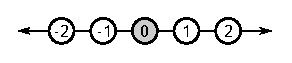
\includegraphics[width=0.6\textwidth]{infinite_drunken.eps}
	\end{center}
	Let the state space consist of all integers.
	Let $X(0) = 0$ (i.e. at time 0 the drunken man is in state 0).
	The transition probabilities are such that
	\[
	P_{i, (i+1)} = P_{i, (i-1)} = 0.5
	\]
	holds for all states $i$ of $\mathbb{X}$.
\end{frame}

\begin{frame}{Gambler's ruin}
\end{frame}

\begin{frame}{Outline}
	\begin{enumerate}
		\item Limiting probabilities
		\item Stationary distribution
		\item Long-run proportion
		\item (Inverse of) Expected return time
	\end{enumerate}
\end{frame}

\begin{frame}{Limiting Probabilities}
	\begin{definition}
		Number $\pi_j$ is the \textit{limiting probability} of $j$ if
		\[
		\pi_j = \lim_{n \to \infty} P^n_{ij}
		\]
		holds for all states $i \in S$ ($S \subseteq \mathbb{N}$ is the state space).
	\end{definition}
	\begin{itemize}
		\item $\pi_j$ is independent of $i$.
		\item $\lim_{n \to \infty} P^n = 
			\begin{pmatrix}
				\pi \\
				\pi \\
				\vdots
			\end{pmatrix}$
			, where $\pi = (\pi_1, \pi_2, \ldots)$
	\end{itemize}
\end{frame}

\begin{frame}{Stationary Probability Distribution}
	\begin{definition}
		Non-negative row vector $\pi = (\pi_1, \pi_2, \ldots)$
		is a \textit{stationary probability distribution} of $\mathbb{X}$
		if $\pi \times P = \pi$ holds and $\sum_{i \in S} \pi_i = 1$
	\end{definition}
	\begin{itemize}
		\item $\pi$ is a normalized left eigenvector with eigenvalue $=1$.
		\item If $X(0)$ has distribution $\pi$, then $X(t)$ has the same distribution $\pi$
			for all $t \geq 1$.
			$\pi$ is also called as \textit{steady-state distribution}.
		\item It doesn't mean that each $X(t)$ become independent.
			$\pi$ only means the distribution of $X(t)$ when the previous random variable's value is unknown.
	\end{itemize}
\end{frame}

\begin{frame}{Theorem 1}
	\begin{theorem}
		Let $\mathbb{X}$ be an \textit{irreducible}, \textit{aperiodic}, \textit{positive recurrent} Markov chain, then
		\begin{itemize}
			\item The limiting probability $\pi_j$ of each state $j$ exists.
			\item $\pi = (\pi_1, \pi_2, \ldots)$ is the unique stationary probability distribution.
		\end{itemize}
	\end{theorem}
	\begin{itemize}
		\item The proof will be stated at page \hyperlink{thm1_proof}{\pageref{thm1_proof}}.
	\end{itemize}
\end{frame}

\begin{frame}{Expected return time}
	\begin{definition}
		The \textit{expected return time} of state $i \in S$ is
		\[
		\mu_i = \sum_{n \geq 1} n \cdot f_i^{(n)}
		\]
		where
		\[
		f_i^{(n)} = P(\min\{t:X(t) = i, t\geq 1\} = n | X(0) = i)
		\]
	\end{definition}
	\begin{itemize}
		\item $f_i = \sum_{n \geq 1} f_i^{(n)}$
	\end{itemize}
\end{frame}

\begin{frame}{Positive recurrent \& null recurrent}
	\begin{definition}
		State $i$ is \textit{positive recurrent} if $\mu_i < \infty$
	\end{definition}
	\begin{definition}
		State $i$ is \textit{null recurrent} if $\mu_i = \infty$
	\end{definition}
	\begin{itemize}
		\item Both are recurrent states, and are \textit{class properties}, which means that if state $i$ and $j$ communicate, they will share this property.
		\item If $\mathbb{X}$ is finite, then each recurrent state of $\mathbb{X}$ is positive recurrent.\\
			Proof stated at page \pageref{finite_pos_rec}.
	\end{itemize}
\end{frame}

\begin{frame}{Example of null recurrent}
	\begin{example}
		For a Markov chain with $n$ states ($1,\ldots,n$), if 
		\[
		P(X(t+1)=i+1|X(t)=i) = 1-1/n
		\]
		and
		\[
		P(X(t+1)=1|X(t)=i) = 1/n
		\]
		According to geometric distribution (taking $p = 1/n$), the expectation value of ``steps taken for state 1 to come back'' will be $1/p = n$, hence $\lim_{n\to\infty} n = \infty$.
	\end{example}
\end{frame}

\begin{frame}{Period of a chain}
	\begin{definition}
		The \textit{period} of state $i$ is $d$ if $d$ is the largest integer such that
		\[
		P^n_{ii} = 0
		\]
		holds for all $n$ which is not divisible by $d$.
	\end{definition}
	\begin{definition}
		If each state of $\mathbb{X}$ has period 1, then $\mathbb{X}$ is called \textit{aperiodic}.
	\end{definition}
	\begin{itemize}
		\item If $P_{ii} > 0$ for all $i \in S$, then $\mathbb{X}$ is aperiodic.
		\item Period can be seen as the $\gcd$ of all $n$ that have $P^n_{ii} > 0$, note that $P^{\gcd}_{ii} > 0$ is not necessary.
		\item The period of drunken man problem is 2.
	\end{itemize}
\end{frame}

\begin{frame}{Lemma 1}
	\begin{lemma}
		If state $j$ has period $1$ and is positive recurrent, then
		\[
		\pi_{ij} \equiv \lim_{n \to \infty} P^n_{ij}
		\]
		exists and is positive for all states $i \in S$.
	\end{lemma}
	\begin{itemize}
		\item This can be proved by the Blackwell theorem in Renewal theory.
		\item It doesn't promise that $\pi_{ij} = \pi_{i'j}$ for any $i,i' \in S$.
			But they will be the same if we add the irreducible property ($i \leftrightarrow i'$).
	\end{itemize}
\end{frame}

\begin{frame}{Property of $\lim$}
	\begin{itemize}
		\item The position of $\lim$ may not be switched arbitrarily in an equation.
			\begin{example}
				\[
				1 = \lim_{n \to \infty}\lim_{m \to \infty} \frac{m}{m+n} \neq
				\lim_{m \to \infty}\lim_{n \to \infty} \frac{m}{m+n} = 0
				\]
			\end{example}
		\item $\lim$ would not influence the inequality.
			\begin{example}
				\begin{center}
					If $f(n) \geq g(n)$, then
					$\lim_{n \to \infty} f(n) \geq \lim_{n \to \infty} g(n)$
				\end{center}
			\end{example}
	\end{itemize}
\end{frame}

\begin{frame}{Property of $\lim$ (cont.)}
	\begin{itemize}
		\item $\lim$ is linear operator under finite number of functions.
	\end{itemize}
	\begin{example}
		For $m < \infty$,
		\[
		\sum_{i=1}^m \lim_{n \to \infty} f_i(n) = \lim_{n \to \infty} \sum_{i=1}^m f_i(n)
		\]
	\end{example}
	\textcolor{red}{need an example of $m = \infty$}
%	\begin{itemize}
%		\item It may not work if we push $m$ to $\infty$ first, since $\sum_{i=1}^m f_i(n)$ may influence the result.
%			For example, if $1 \leq i \leq n, f_i(n) = 1/n$, then LHS will be 0, while RHS will be 1.
%			But pushing $m$ to $\infty$ after pushing $n$ to $\infty$ first is OK.
%	\end{itemize}
\end{frame}

\begin{frame}{Inequality 1}
	\begin{ineq}
		\[
		\sum_{j \in S} \pi_{ij} \leq 1 \quad\forall i \in S
		\]
	\end{ineq}
\end{frame}

\begin{frame}{Proof}
		\begin{align*}
			\lim_{m \to \infty} \sum_{j=1}^m \pi_{ij} &= \lim_{m \to \infty} \sum_{j=1}^m \lim_{n \to \infty} P^n_{ij} \\
			&= \lim_{m \to \infty} \lim_{n \to \infty} \sum_{j=1}^m P^n_{ij} \\
			&\leq \lim_{m \to \infty} \lim_{n \to \infty} \sum_{j \in S} P^n_{ij} = 1
		\end{align*}
	\begin{itemize}
		\item The last equation works since $\sum_{j \in S} P^n_{ij} = 1$.
	\end{itemize}
\end{frame}

\begin{frame}{Inequality 2}
	\begin{ineq}
		For state $j \in S$, we have
		\[
		\pi_{ij} \geq \sum_{k \in S} \pi_{ik} P_{kj}
		\]
	\end{ineq}
\end{frame}

\begin{frame}{Proof}
	For $m \geq 1$ and $n \geq 1$,
	\[
	P^{n+1}_{ij} = \sum_{k \in S} P^n_{ik} P_{kj} \geq \sum_{k=1}^m P^n_{ik} P_{kj}
	\]
	then
	\[
	\pi_{ij} = \lim_{n \to \infty} P^{n+1}_{ij}
		\geq \lim_{n \to \infty} \sum_{k=1}^m P^n_{ik} P_{kj} 
		 = \sum_{k=1}^m \lim_{n \to \infty} P^n_{ik} P_{kj} 
		 = \sum_{k=1}^m \pi_{ik} P_{kj}
	\]
	hence, we know
	\[
	\lim_{m\to\infty} \pi_{ij} = \pi_{ij} \geq 
	\lim_{m\to\infty}\sum_{k=1}^m \pi_{ik}P_{kj} = \sum_{k\in S} \pi_{ik}P_{kj}
	\]
\end{frame}

\begin{frame}{Equality 1}
	\begin{eq}
		\[
		\pi_{ij} = \sum_{k \in S} \pi_{ik} P_{kj}
		\]
	\end{eq}
\end{frame}

\begin{frame}{Proof}

		Assume for contradiction $\pi_{ij} > \sum_{k \in S} \pi_{ik} P_{kj}$, then
		\begin{align*}
		\lim_{m\to\infty}\sum_{j=1}^m & > \lim_{m\to\infty}\sum_{j=1}^m 
		\lim_{p\to\infty}\sum_{k=1}^p \pi_{ik}P_{kj} \\
		& = \lim_{m\to\infty}\lim_{p\to\infty}\sum_{j=1}^m \sum_{k=1}^p \pi_{ik}P_{kj} \\
		& = \lim_{m\to\infty}\lim_{p\to\infty}\sum_{k=1}^p \pi_{ik} \sum_{j=1}^m P_{kj} \\
		& = \lim_{p\to\infty}\sum_{k=1}^p \pi_{ik} \lim_{m\to\infty}\sum_{j=1}^m P_{kj} \\
		& = \lim_{p\to\infty}\sum_{k=1}^p \pi_{ik} \cdot 1 = \lim_{p\to\infty}\sum_{k=1}^p \pi_{ik}
		\end{align*}
		
%		\begin{align*}
%			\sum_{j \in S} \pi_j &> \sum_{j \in S}\sum_{i \in S} \pi_i P_{ij} \\
%			&= \sum_{i \in S} \pi_i \sum_{j \in S} P_{ij} = \sum_{i \in S} \pi_i
%		\end{align*}
		

%	\begin{itemize}
%		\item $\sum$ should be represented by $\lim \sum$, the equation will still work.
%		\item \textcolor{red}{why the proof work when switching $\sum_{j \in S} \& \sum_{i \in S}$?}
%	\end{itemize}
\end{frame}

\begin{frame}{Proof (cont.)}
\begin{itemize}
\item Since a value cannot be greater than itself, we got contradiction.
\item In the 4th line, two $\lim$ can be switched because the value can only get larger when applying $\lim$ on it. \textcolor{red}{not sure}
\end{itemize}
\end{frame}

\begin{frame}{Proof of theorem 1}\label{thm1_proof}
	\begin{itemize}
		\item \textbf{Step 0}: existence of limiting probability.
		\item \textbf{Step 1}: existence of stationary probability distribution.
		\item \textbf{Step 2}: uniqueness.
	\end{itemize}
\end{frame}

\begin{frame}{0. Existence of limiting probability}
	\begin{proof}
		By lemma 1, we know that there exists a $\pi_j$ for row $i$.
		Since the Markov chain is irreducible and all the states are positive recurrent, 
		for any state $i'$ other than $i$, we know that $i'$ surely will visit $i$ in finite steps.
		Therefore, the $\pi_j$ value at row $i'$ will equal to the $\pi_j$ value at row $i$,
		which means that all the $\pi_j$ for column $j$ are the same, and is the limiting probability.
	\end{proof}
	\textcolor{red}{still not clear enough}
\end{frame}

\begin{frame}{1. Existence of stationary probability distribution}\label{existence}
	We want to prove that
	\begin{target}
		There's a vector $s = (s_1, s_2, \ldots)$ such that
		\begin{enumerate}
			\item $\sum_{i \in S} s_i = 1$
			\item $s \times P = s$
		\end{enumerate}
	\end{target}
\end{frame}

\begin{frame}
	\begin{proof}
		By lemma 1, we know that there exists a $\pi = (\pi_1, \pi_2, \ldots)$. \\
		And by equality 1, we know that
		\[
		(\pi_1, \pi_2, \ldots) \times P = (\pi_1, \pi_2, \ldots)
		\]
		Hence $\pi$ can satisfy the 2nd part of our target. \\
		Then, we take $k = \sum_{i \in S} \pi_i$.
		By inequality 1, we know that $k < \infty$, and can get
		\[
		(\frac{\pi_1}{k}, \frac{\pi_2}{k}, \ldots) \times P = (\frac{\pi_1}{k}, \frac{\pi_2}{k}, \ldots)
		\]
		where $\sum_{i \in S} \frac{\pi_i}{k} = 1$ also satisfy the 1st part of our target. \\
		Therefore, this vector can be $s$, which means that it exists.
	\end{proof}
\end{frame}

\begin{frame}{2. Uniqueness}\label{uniqueness}
	\begin{target}
		If $s = (s_1, s_2, \ldots)$ is a stationary distribution of $\mathbb{X}$, then $s = \pi$.
	\end{target}
	\begin{itemize}
		\item We'll prove this by inequality 3 \& 4.
	\end{itemize}
\end{frame}

\begin{frame}{Inequality 3}
	\begin{ineq}
		\[
		s_j \geq \pi_j, \forall j \in S
		\]
	\end{ineq}
\end{frame}

\begin{frame}
	\begin{proof}
		Let the distribution of $X(0)$ be $s$, by the property of stationary distribution, we have
		\begin{align*}
			             s_j &= P(X(n)=j) = \sum_{i \in S} P(X(n) = j | X(0) = i)P(X(0) = i) \\
			                 &= \sum_{i \in S} P^n_{ij} \cdot s_i \\
			                 &\geq \sum_{i=1}^m P^n_{ij} \cdot s_i \\
			\Rightarrow  s_j &= \lim_{m \to \infty}\lim_{n \to \infty} s_j \\
			                 &\geq \lim_{m \to \infty}\lim_{n \to \infty} \sum_{i=1}^m P^n_{ij} \cdot s_i
			                  = \lim_{m \to \infty}\sum_{i=1}^m \pi_j \cdot s_i = \pi_j
		\end{align*}
	\end{proof}
\end{frame}

\begin{frame}{Inequality 4}
	\begin{ineq}
		\[
		s_j \leq \pi_j, \forall j \in S
		\]
	\end{ineq}
\end{frame}

\begin{frame}
	\begin{proof}
		Similar in the proof above, $\forall m,n \geq 1$, we have
		\begin{align*}
			            s_j &= \sum_{i \in S} P^n_{ij} \cdot s_i \\
			                &\leq \sum_{i=1}^m P^n_{ij} \cdot s_i + \sum_{i=m+1}^\infty s_i \\
			\Rightarrow s_j &= \lim_{m \to \infty}\lim_{n \to \infty} s_j \\
			                &\leq \lim_{m \to \infty}\lim_{n \to \infty} \left( 
			                	\sum_{i=1}^m P^n_{ij} \cdot s_i + \sum_{i=m+1}^\infty s_i \right) \\
			                &= \pi_j
		\end{align*}
	\end{proof}
\end{frame}

\begin{frame}{An example Markov chain}
	\begin{example}
		\[
		P = 
		\begin{pmatrix}
			\alpha & 1 - \alpha \\
			\beta  & 1 - \beta
		\end{pmatrix},
		0 < \alpha, \beta < 1
		\]
		\[
		\pi = \left( \frac{\beta}{1+\beta-\alpha}, \frac{1-\alpha}{1+\beta-\alpha} \right) 
		\]
	\end{example}
\end{frame}

\begin{frame}{Real world example: Hardy-Weinberg Law}
	\begin{example}
		There're two kinds of allele: 
		\begin{itemize}
			\item dominant: \textbf{A}
			\item recessive: \textbf{a}
		\end{itemize}
		And three kinds of senotype with population proportion as follow:
		\begin{itemize}
			\item AA: $p$
			\item aa: $q$
			\item Aa: $r = 1 - (p + q)$
		\end{itemize}
	\end{example}
\end{frame}

\begin{frame}
	\begin{example}[cont.]
		\[
		P = 
		\bordermatrix{ ~ & AA                      & aa                      & Aa            \cr
			            AA & p+\frac{r}{2}           & 0                       & q+\frac{r}{2} \cr
			            aa & 0                       & q+\frac{r}{2}           & p+\frac{r}{2} \cr
			            Aa & \frac{p}{2}+\frac{r}{4} & \frac{p}{2}+\frac{r}{4} & \frac{p+q+r}{2} \cr}
		\]
		we get $\pi = (p, q, r)$ when
		\begin{itemize}
			\item $p = {\left( p + \frac{r}{2} \right)}^2$
			\item $q = {\left( q + \frac{r}{2} \right)}^2$
			\item $r = 2 \left( p + \frac{r}{2} \right)\left( q + \frac{r}{2} \right)$
		\end{itemize}
	\end{example}
\end{frame}

\begin{frame}{Long-run proportion}
	\begin{definition}
		We say that $r_j$ is the \textit{long-run proportion} of state $j \in S$ if
		\[
		r_j = \lim_{n\to\infty} \frac{1}{n} \sum_{1 \leq t \leq n} P^t_{ij}
		\]
		holds for each state $i \in S$.
	\end{definition}
	\begin{itemize}
		\item It represents the average appearance times of state $j$ in the whole process.
		\item We will show that (in theorem 3) if $\mathbb{X}$ is irreducible, then the long-run proportion of all states exist.
	\end{itemize}
\end{frame}

\begin{frame}{Theorem 2}
	\begin{theorem}[type 1]
	If $r_j$ exists for each $j \in S$ and $\sum_{j \in S} r_j > 0$,
	then $r = (r_1, r_2, \ldots)$ is the unique stationary distribution of $\mathbb{X}$.
	\end{theorem}
	or
	\begin{theorem}[type 2]
	If $r_j$ exists for each $j \in S$ and \textbf{a stationary distribution exists},
	then $r = (r_1, r_2, \ldots)$ is the unique stationary distribution of $\mathbb{X}$.
	\end{theorem}
\end{frame}

\begin{frame}[shrink]{Proof}
	\textbf{Existence of stationary distribution in type 1:} \\
	Let 
	\[
	R = 
	\begin{pmatrix}
		r \\
		r \\
		\vdots
	\end{pmatrix} 
	= \lim_{n\to\infty} \frac{1}{n} \sum_{1 \leq t \leq n} P^t
	\]
	then
	\begin{align*}
		R \times P &= \lim_{n\to\infty} \frac{1}{n} \sum_{1 \leq t \leq n} P^{t+1} \\
		&= \lim_{n\to\infty} \frac{1}{n} \sum_{1 \leq t \leq n} P^t + \lim_{n\to\infty} \frac{1}{n}(P^{n+1} - P) \\
		&= R
	\end{align*}
	As stated later, $\sum_{j \in S} r_j \leq 1$, hence by normalizing $r$, we prove that stationary distribution exist.
	\begin{itemize}
	\item \textcolor{red}{$(\lim f(n))\cdot g(n) = \lim f(n) \cdot g(n)$?}
	\item \textcolor{red}{can replace the proof on page \pageref{existence}?}
	\end{itemize}
\end{frame}

\begin{frame}{Proof (cont.)}
	\textbf{Uniqueness:} \\
	Let $\pi$ be an arbitrary stationary distribution, then
	\begin{align*}
	r &= \pi \times R \\
	&= \pi \times \lim_{n\to\infty} \frac{1}{n} \sum_{1 \leq t \leq n} P^t \\
	&= \lim_{n\to\infty} \frac{1}{n} \sum_{1 \leq t \leq n} \pi \times P^t \\
	&= \lim_{n\to\infty} \frac{1}{n} \sum_{1 \leq t \leq n} \pi \\
	&= \pi
	\end{align*}
	\textcolor{red}{can replace the proof for page \pageref{uniqueness}?}
\end{frame}

\begin{frame}{Proof (cont.)}\label{proportion_sum}
	\textbf{Prove that $\sum_{j \in S} r_j \leq 1$:}\\
	\begin{align*}
	\sum_{j \in S} r_j & = 
	\lim_{m\to\infty} \sum_{j=1}^m \lim_{n\to\infty} \frac{1}{n} \sum_{t=1}^n P^t_{ij} \\
	& = \lim_{m\to\infty} \lim_{n\to\infty} \frac{1}{n}\sum_{t=1}^n \sum_{j=1}^m P^t_{ij} \\
	& \leq \lim_{m\to\infty} \lim_{n\to\infty} \frac{1}{n}\sum_{t=1}^n \sum_{j\in S} P^t_{ij} \\
	& = \lim_{m\to\infty} \lim_{n\to\infty} \frac{1}{n}\sum_{t=1}^n 1 = 1
	\end{align*}
\end{frame}

\begin{frame}{Example 1}
	On a highway, if we know the probability that
	\begin{itemize}
	\item A truck is followed by a truck: $1/4$
	\item A truck is followed by a car: $3/4$
	\item A car is followed by a truck: $1/5$
	\item A car is followed by a car: $4/5$
	\end{itemize}
	We can construct a matrix
	\[
	\bordermatrix{~ & T   & C   \cr
                  T & 1/4 & 3/4 \cr
                  C & 1/5 & 4/5 \cr}
	\]
	and get the portion of trucks and cars on the whole highway as the eigenvector $(4/19, 15/19)$
	(we will know that long-run proportion exists by Theorem 3).
\end{frame}

\begin{frame}{Example 2}
	For a system which has several good and bad states, we have a matrix $P$:
	\[
	\bordermatrix{~      & g_1 & g_2 & \cdots & b_1 & b_2 & \cdots \cr
                  g_1    &     &     &        &     &     &        \cr
                  g_2    &     &     &        &     &     &        \cr
                  \vdots &     &     &        &     &     &        \cr
                  b_1    &     &     &        &     &     &        \cr
                  b_2    &     &     &        &     &     &        \cr
                  \vdots &     &     &        &     &     &        \cr}
	\]
\end{frame}

\begin{frame}{Example 2 (cont.)}
	\textbf{Q1:} Breakdown rate (breakdown times $/$ total time)\\
	The long-run frequency of going to a bad state from a good state is
	\[
	\sum_{i \in g} \sum_{j \in b} r_i P_{ij}
	\]
\end{frame}

\begin{frame}{Example 2 (cont.)}
	\textbf{Q2:} The expected time $\mu_G$ (resp. $\mu_B$) of staying in good (resp. bad) states once we reach a good (resp. bad) state? \\
	\textbf{Ans:} \\
	For each $t = 1, 2, \ldots$, let $G_t$ (resp. $B_t$) be the length of the $t$-th good (resp. bad) phase of consecutive good (resp. bad) states.
	By the strong law of large numbers, 
	\[
	P\left( \lim_{t\to\infty} \frac{G_1 + B_1 + G_2 + B_2 + \cdots + G_t + B_t}{t} = \mu_G + \mu_B \right) = 1
	\]
	Since the reciprocal of above is the breakdown rate, we get equation (1):
	\[
	P\left( \sum_{i \in G} \sum_{j \in B} \pi_i P_{ij} = \frac{1}{\mu_G + \mu_B} \right) = 1
	\]
\end{frame}

\begin{frame}{Example 2 (cont.)}
	Also, with probability 1, we get equation (2):
	\[
	P\left( \sum_{i \in G} r_i = 
	\lim_{t\to\infty}\frac{G_1 + G_2 + \cdots + G_t}{G_1 + B_1 + \cdots + G_t + B_t}
	= \frac{\mu_G}{\mu_G + \mu_B} \right) = 1
	\]
	Then, by $(2)/(1)$, we get that
	\[
	P\left( \mu_G = \frac{\sum_{i \in G} r_i}{\sum_{i \in G}\sum_{j \in B} r_i P_{ij}} \right) = 1
	\]
	\begin{itemize}
	\item \textcolor{red}{$\lim \frac{f(n)}{g(n)} = \frac{\lim f(n)}{\lim g(n)}$?}
	\end{itemize}
\end{frame}

\begin{frame}{Theorem 3}\label{pro_value}
	\begin{theorem}
	If $\mathbb{X}$ is irreducible, then the long-run proportion $r_i$ exists with probability $1$, moreover,
	\begin{enumerate}
	\item If state $i$ is positive recurrent (i.e. $0 < \mu_i < \infty$), then $P(r_i = \frac{1}{\mu_i}) = 1$.
	\item If state $i$ is null recurrent (i.e. $\mu_i = \infty$) or transient, then $P(r_i = 0) = 1$.
	\end{enumerate}
	where $\mu_i$ is the expected return time of state $i$
	\end{theorem}
\end{frame}

\begin{frame}{Proof}
	\textbf{Part 1:} \\
	Suppose $X(0) = i$, $T_k$ is the number of steps required for the $k$-th $i$ goes to $(k+1)$-st $i$,
	then by the strong law of large number,
	\begin{align*}
	&P\left( \lim_{k\to\infty} \frac{T_1 + T_2 + \cdots + T_k}{k} = \mu_i \right) = 1 \\
	\Rightarrow & P\left( r_i = \lim_{k\to\infty} \frac{k}{T_1 + T_2 + \cdots + T_k} = \frac{1}{\mu_i} \right) = 1
	\end{align*}
	\begin{itemize}
	\item \textcolor{red}{$\lim (A/B) = \frac{1}{\lim (B/A)}$?}
	\end{itemize}
\end{frame}

\begin{frame}{Proof (cont.)}
	\textbf{Part 2:} \\
	\begin{enumerate}
	\item If $i$ is transient, $i$ will only appear finite times in the long-run, hence
		\[
		r_i = \frac{finite}{\infty} = 0
		\]
	\item If $i$ is null recurrent, $\mu_i$ is $\infty$, then
		\[
		P\left( \lim_{k\to\infty} \frac{T_1 + T_2 + \cdots + T_k}{k} = \infty \right) = 1
		\]
		\[
		P\left( r_i = \lim_{k\to\infty} \frac{k}{T_1 + T_2 + \cdots + T_k} = 0 \right) = 1
		\]
		(The first equation is not promised by the strong law of large number.
		But if it's not $\infty$, we can say that $\mu_i$ is not $\infty$, which is a contradiction.)
	\end{enumerate}
\end{frame}

\begin{frame}{Example 1}\label{finite_pos_rec}
	\begin{example}[type 1]
	If $\mathbb{X}$ is \textbf{irreducible} and finite, then $\mathbb{X}$ has no null recurrent states.
	\end{example}
	\begin{example}[type 2]
	If $\mathbb{X}$ is finite, then $\mathbb{X}$ has no null recurrent states.
	\end{example}
	\begin{itemize}
	\item Finite irreducible imply positive recurrent.
	\end{itemize}
\end{frame}

\begin{frame}{Proof}
	\begin{itemize}
	\item \textbf{Type 1:}\\
		If there's a state which is null recurrent, by irreducible, all the states will be null recurrent.
		Then, all states have $P(r_i = 0) = 1$.
		By changing the proof in page \pageref{proportion_sum} into finite states version, 
		we know that $\sum r_i = 1$.
		So it's impossible for finite $r_i$, which are all close to 0, to sum up to 1.
	\item \textbf{Type 2:}\\
		If it's not irreducible, the finite set of communicated null recurrent states still form an irreducible and finite Markov chain, which can fit the requirement of type 1.
	\end{itemize}
\end{frame}

\begin{frame}{Example 2}
	\begin{example}
	In the drunken man problem with infinite states, no state will be positive recurrent.
	\end{example}
	\begin{itemize}
	\item Infinite drunken man imply no positive recurrent.
		Note that it doesn't mean all infinite irreducible Markov chain has no positive recurrent state.
	\end{itemize}
\end{frame}

\begin{frame}{Proof}
	If all the states are positive recurrent, then by theorem 3, 
	we know that all the $r_i > 0$ and is a finite value.
	Since each state of drunken man problem has the same structure, all the $r_i$ has same value.
	We then set $r = \epsilon\cdot r_i$ ($0 < \epsilon < 1$) such that 
	$r_i > r > 0, \forall i$.
	And get
	\[
	\sum_{i\in S} r_i > \sum_{i\in S} r = \infty > 1
	\]
	which is contradiction to \hyperlink{proportion_sum}{page \pageref{proportion_sum}}.
\end{frame}

\begin{frame}{Example 3: Poisson Hotel}
	\begin{example}
	There's a hotel, with $N$ representing the number of newly occupied rooms each day ($N$ is a poisson distribution with parameter $\lambda$).
	And the number of consecutive check-in days of each room is a geometric distribution with probability $p$ ($p$ is the probability of check-out).
	$X(t)$ is the number of occupied rooms in day $t$.
	\end{example}
\end{frame}

\begin{frame}{\textbf{Q1:} $P_{ij} = $?}
	We set $R_i$ as a binomial distribution with parameter $(i, 1-p)$, which represents the number of rooms which will remain occupied in the next day, then
	\begin{align*}
	P_{ij} & = P(R_i + N = j) \\
	& = \sum_{k\geq 0} P(R_i + N = j | R_i = k)P(R_i = k) \\
	& = \sum_{k\geq 0} P(N = j-k)P(R_i = k) \\
	& = \sum_{0 \leq k \leq \min(i,j)} \frac{e^{-\lambda}\cdot \lambda^{j-k}}{(j-k)!} \binom{i}{k} (1-p)^k p^{1-k}
	\end{align*}
\end{frame}

\begin{frame}{\textbf{Q2:} $r_i =$?}
	We guess (by a dream?) there's a stationary distribution which is a poisson distribution with parameter $\lambda_0$.
	Setting $X(0)$ with this distribution. 
	And let $R$ as the number of rooms in $X(0)$ which remain check-in in the next day ($R$ is a poisson distribution with parameter $\lambda_0 (1-p)$).
	$X(1)$ will have distribution $R + N$, which is a poisson distribution with parameter $\lambda_0 (1-p) + \lambda$.
	Then since $X(0)$ is a stationary distribution, it will have the same distribution with $X(1)$, which means that $\lambda_0 = \lambda_0 (1-p) + \lambda$, and we get $\lambda_0 = \lambda / p$.
	
	After getting $r_i$, we get that with probability 1, 
	\[
	\mu_i = \frac{1}{P(X(0)=i)} = \frac{i!}{e^{-\lambda/p}\cdot (\lambda/p)^i}
	\]
	\textcolor{red}{not clear enough}
\end{frame}

\begin{frame}{Corollary of theorem 2 \& 3}
\begin{corollary}
If $\mathbb{X}$ is irreducible, then
\[
\text{$\mathbb{X}$ is positive recurrent $\iff \mathbb{X}$ admits a stationary distribution.}
\]
\end{corollary}
\end{frame}

\begin{frame}{Moving to transient states}
For transient states $i$ and $j$, we define the following:
\begin{enumerate}
\item Expected steps in a transient state:
	\begin{definition}
	$E$ is a matrix where $E_{ij}$ is the expected number of steps $t$ with $X(t) = j$ when $X(0)=i$.
	\end{definition}
\item Probability of reaching a transient state:
	\begin{definition}
	$F$ is a matrix where
	\[
	F_{ij} = P(X(t)=j \text{ for some } t \geq 1 | X(0)=i)
	\]
	\end{definition}
\end{enumerate}
\end{frame}

\begin{frame}{Computing $E$ \& $F$}
\begin{theorem}
For a Markov chain $\mathbb{X}$ consisting finite transient states,
\[
E = (I - T)^{-1}
\]
where $I$ is an identity matrix, $T$ is the induced matrix of $P$ by all the transient states in $P$.
Moreover,
\[
F_{ij} = \frac{E_{ij} - \delta_{ij}}{E_{jj}} ~\text{,where}~ \delta_{ij}=
\begin{cases}
1 & \text{if } i=j \\
0 & \text{if } i \neq j
\end{cases}
\]
\end{theorem}
\end{frame}

\begin{frame}{Proof}
Conditioned on $X(1)$, we have
\[
E_{ij} = \underbrace{\delta_{ij}}_{\text{step} = 0} + 
	\underbrace{\sum_k P_{ik} \cdot E_{kj}}_{\text{step} \geq 1}
	= \delta_{ij} + \sum_k T_{ik} \cdot E_{kj}
\]
The 2nd equation works since the process will not go back to transient state once it enter a recurrent state.
Then, we have
\begin{align*}
& I \times E = E = I + T \times E \\
\implies & (I - T) \times E = I \\
\implies & E = (I - T)^{-1}
\end{align*}
\end{frame}

\begin{frame}{Proof (cont.)}
Conditioned on whether or not $X(t) = j$ holds for some $t \geq 1$, we have
\[
E_{ij} = \underbrace{\delta_{ij}}_{\text{step} = 0} + 
	\underbrace{F_{ij} \cdot E_{jj}}_{\text{steps $\geq$ the first $j$}}
\]
therefore,
\[
F_{ij} = \frac{E_{ij} - \delta_{ij}}{E_{jj}}
\]
\end{frame}

\begin{frame}{Example: Gambler's ruin}
\begin{center}
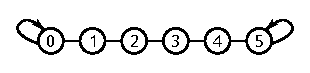
\includegraphics[scale=1.5]{gambler_line}
\end{center}
\[
T = \bordermatrix{~ & 1   & 2   & 3   & 4 \cr
                  1 & 0   & 0.5 & 0   & 0 \cr
                  2 & 0.5 & 0   & 0.5 & 0 \cr
                  3 & 0   & 0.5 & 0   & 0.5 \cr
                  4 & 0   & 0   & 0.5 & 0 \cr}
~E = \begin{pmatrix}
1.6 & 1.2 & 0.8 & 0.4 \\
1.2 & 2.4 & 1.6 & 0.8 \\
0.8 & 1.6 & 2.4 & 1.2 \\
0.4 & 0.8 & 1.2 & 1.6
\end{pmatrix}
\]
\[
F = \begin{pmatrix}
0.375 & 0.5 & 1/3 & 0.25 \\
0.75 & 1.75/3 & 1.9/3 & 0.5 \\
0.5 & 1.9/3 & 1.75/3 & 0.75 \\
0.25 & 1/3 & 0.5 & 0.375
\end{pmatrix}
\]
\end{frame}

\begin{frame}{Branching process}
In the beginning, there're $X(0)$ life forms, 
each life form has probability $p_i$ of becoming $i$ life forms in the next step.
\begin{itemize}
\item state 0 is recurrent (absorbing).
\item if $p_0 > 0$, all other states ($1,2,\ldots$) are transient since\\
	$P(X(t+1)=0|X(t)=i) = {p_0}^i > 0$
\end{itemize}
We'll show that
\[
E[X(n)] = \mu^n \cdot X(0)
\]
where
\[
\mu = \sum_{j \geq 1} j \cdot p_j = E[Z_k]
\]
and $Z_k$ is the number of offspring of the $k$-th life form, all $Z_k$ are i.i.d.
\end{frame}

\begin{frame}{Proof}
\begin{align*}
E[X(n)] & = E[E[X(n)|X(n-1)]] \\
& = E\left[E\left[\sum_{k=1}^{X(n-1)} Z_k | X(n-1)\right]\right] \\
& = E[X(n-1) \cdot \mu] \\
& = \mu \cdot E[X(n-1)] \\
& = \mu^n \cdot X(0)
\end{align*}
\end{frame}

\begin{frame}{Probability of extinction}
\begin{definition}
$e_i$ is the probability of extinction when $X(0) = i$.
\end{definition}
\textbf{Case 1:} $\mu < 1$
\begin{align*}
1 - e_i & = \lim_{n\to\infty} P(X(n) \geq 1 | X(0) = i) \\
& = \lim_{n\to\infty} \sum_{j \geq 1} P(X(n) = j|X(0) = i) \\
& \leq \lim_{n\to\infty} \sum_{j \geq 1} j \cdot P(X(n) = j|X(0) = i) \\
& = \lim_{n\to\infty} E[X(n)|X(0)=i] \\
& = \lim_{n\to\infty} \mu^n \cdot i = 0
\end{align*}
\end{frame}

\begin{frame}{Probability of extinction (cont.)}
\textbf{Case 2:} $\mu \geq 1$ 
\[
e_2 = {e_1}^2,\quad  e_3 = e_2 \cdot e_1,\quad\ldots
\]
\begin{align*}
e_1 & = P(\text{extinct}|X(0) = 1) \\
& = \sum_{j \geq 0} P(\text{extinct}|X(1) = j) \cdot P_{1j} \\
& = \sum_{j \geq 0} e_j \cdot p_j \\
& = \sum_{j \geq 0} {e_1}^j \cdot p_j
\end{align*}
We then solve the above equation to get $e_1$.
\end{frame}

\begin{frame}{Example}
\begin{align*}
& p_0 = p_1 = 0.25,\quad p_2 = 0.5 \\
\implies & \mu = 1 \cdot 0.25 + 2 \cdot 0.5 > 1 \\
\implies & e_1 = {e_1}^0 \cdot 0.25 + {e_1}^1 \cdot 0.25 + {e_1}^2 \cdot 0.5 \\
\implies & e_1 = \{1/2,~1\}
\end{align*}
Since $\mu > 1$, we know $\lim_{n\to\infty} E[X(n)] = \infty$.\\
But if $e_1 = 1$, we have $\lim_{n\to\infty} P(X(n) = 0) = 1$, which would not make $\lim_{n\to\infty} E[X(n)] = \infty$, hence $e_1 \neq 1$.
\end{frame}

\begin{frame}{Reversed Markov chain}
\begin{definition}
Let $\mathbb{X}$ (resp. $\mathbb{Y}$) be a Markov chain with matrix $P$ (resp. $Q$).\\
We say that $\mathbb{Y}$ is the \textit{reversed chain} of $\mathbb{X}$ if there exists a stationary distribution $\pi$ of $\mathbb{X}$ such that
\[
\pi_i \cdot Q_{ij} = \pi_j \cdot P_{ji}
\]
holds for all states $i,~ j \in S$.
\end{definition}
\end{frame}

\begin{frame}{Observation 1}
\begin{obs}
The reversed sequence $\mathbb{Y}$ of $\mathbb{X}$ is a Markov chain.
\end{obs}
\end{frame}

\begin{frame}{Proof}
\begin{align*}
& P(Y(n) = i_0 | Y(n-1) = i_1, Y(n-2) = i_2, \ldots , Y(n-k) = i_k) \\
= & P(X(n) = i_0 | X(n+1) = i_1, X(n+2) = i_2, \ldots , X(n+k) = i_k) \\
= & \frac{P(X(n) = i_0, X(n+1) = i_1, \ldots , X(n+k) = i_k)}{P(X(n+1) = i_1, \ldots , X(n+k) = i_k)} \\
= & \frac{P(X(n)=i_0)\cdot P(X(n+1)=i_1|X(n)=i_0)\cdot P_{i_1 i_2}\cdots P_{i_{k-1}i_k}}{P(X(n+1)=i_1)\cdot P_{i_1 i_2}\cdots P_{i_{k-1}i_k}} \\
= & \frac{P(X(n)=i_0, X(n+1)=i_1)}{P(X(n+1)=i_1)} \\
= & P(X(n)=i_0|X(n+1)=i_1) \\
= & P(Y(n)=i_0|Y(n-1)=i_1)
\end{align*}
\end{frame}

\begin{frame}{Observation 2}
\begin{obs}
If $\mathbb{Y}$ is the reversed sequence of Markov chain $\mathbb{X}$ and $\pi$ is a stationary distribution of $\mathbb{X}$, then
\[
\pi_i \cdot Q_{ij} = \pi_j \cdot P_{ji}
\]
holds for all $i,j \in S$, where $Q$ is the transition matrix of $\mathbb{Y}$.
\end{obs}
\end{frame}

\begin{frame}{Proof}
Let $\mathbb{X}$ and $\mathbb{Y}$ have distribution $\pi$
\begin{align*}
\pi_i \cdot Q_{ij} & = P(Y(n-1)=i)\cdot P(Y(n)=j|Y(n-1)=i) \\
& = P(Y(n-1)=i, Y(n)=j) \\
& = P(Y(n-1)=i|Y(n)=j)\cdot P(Y(n)=j) \\
& = P(X(n+1)=i|X(n)=j)\cdot P(X(n)=j) = \pi_j \cdot P_{ji}
\end{align*}
\end{frame}

\begin{frame}{Observation 3}\label{obs3}
\begin{obs}
Let $P$ (resp. $Q$) be the transition matrix of $\mathbb{X}$ (resp. $\mathbb{Y}$),
if vector $\pi$ satisfy the following
\begin{itemize}
\item $\sum_{i\in S} \pi_i = 1$
\item $\pi_i \geq 0 \quad\forall i \in S$
\item $\pi_i \cdot Q_{ij} = \pi_j \cdot P_{ji} \quad\forall i,j \in S$
\end{itemize}
then $\mathbb{Y}$ is the reversed sequence of $\mathbb{X}$.
\end{obs}
\begin{itemize}
\item The long-run proportion of $i\to j$ in the sequence of $\mathbb{Y}$ is equal to the long-run proportion of $j\to i$ in the sequence of $\mathbb{X}$.
\item Reversed Markov chain is the reversed sequence.
\end{itemize}
\end{frame}

\begin{frame}{Proof}
From the third property, we have
\[
\sum_{j\in S} \pi_i \cdot Q_{ij} = \pi_i = \sum_{j\in S} \pi_j \cdot P_{ji} \quad\forall i \in S
\]
From the 2nd equation, we know that $\pi \times P = \pi$, hence $\pi$ is a stationary distribution of $\mathbb{X}$.

Then by observation 2, we know that for any $\pi$, there's a reversed sequence $\mathbb{Y}'$, whose transition matrix $Q'$ satisfy
\[
\pi_i \cdot Q_{ij}' = \pi_j \cdot P_{ji} \quad\forall i,j \in S
\]
hence $\mathbb{Y} = \mathbb{Y}'$, which is a reversed sequence of $\mathbb{X}$.
\end{frame}

\begin{frame}{Example: Bulb's life}
\begin{center}

\includegraphics[scale=0.1]{light_bulb_1.png}
\end{center}
There's a room which need to be lighted by one bulb, when the bulb in use fails, it will be replaced by a new one on next day.
\begin{itemize}
\item $X(n) = i$ if the bulb in use on day $n$ is in its $i$th day of use.
\item $L$ is a random variable representing the lifetime of a bulb.
\end{itemize}
We want to know the stationary probability $\pi_i$ of state $i$.
\end{frame}

\begin{frame}{Example: Bulb's life (cont.)}
$\mathbb{X}$ is a irreducible, positive recurrent, aperiodic Markov chain which has the sequence like this:
\[
1,2,3,1,2,3,4,5,1,1,2,1,2,3,4,\ldots
\]
We know that
\[
P_{i1} = P(\text{buld, on its $i$th day of use, fails}) = \frac{P(L=i)}{P(L\geq i)} = 1 - P_{i(i+1)}
\]
And the expected return time of state $1$ is $E[L]$, which means that the long-run proportion of state $1$ is $1/E[L]$ by page \pageref{pro_value}.
\end{frame}

\begin{frame}{Example: Bulb's life (cont.)}
Take $\mathbb{Y}$ (with matrix $Q$) as the reversed chain of $\mathbb{X}$, we know that for all $i\in S$,
\begin{itemize}
\item $Q_{(i+1)i} = 1$
\item $Q_{1i} = P(L = i)$
\item $\pi_1\cdot Q_{1i} = \pi_i\cdot P_{i1}$
\end{itemize}
Hence,
\[
\pi_i = \frac{\pi_1\cdot Q_{1i}}{P_{i1}} = 
\frac{P(L=i)\cdot P(L\geq i)}{E[L]\cdot P(L=i)} = \frac{P(L\geq i)}{E[L]}
\]
\end{frame}

\begin{frame}{Time-reversible}
\begin{definition}
$\mathbb{X}$ is \textit{time-reversible} if $\mathbb{X}$ is the reversed chain of $\mathbb{X}$.
\end{definition}
\end{frame}

\begin{frame}{Example: Reversed drunken man}
\begin{center}
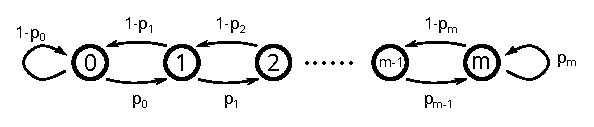
\includegraphics[scale=1.0]{drunken_man}
\end{center}
\begin{itemize}
\item $0 < p_0\leq 1$
\item $0\leq p_m < 1$
\item $0 < p_i < 1 \quad\forall i = 1,\ldots,m-1$
\end{itemize}
The long-run proportion of transition $i\to i+1$ and $i+1\to i$ are the same, since one must go back to $i$ from $i+1$ in order to go to $i+1$ from $i$.\\
Hence the drunken man problem is time-reversible.
\end{frame}

\begin{frame}{Example: Reversed drunken man (cont.)}
\begin{align*}
\pi_0\cdot p_0 &= \pi_1\cdot (1-p_1)\\
\pi_1\cdot p_1 &= \pi_2\cdot (1-p_2)\\
&\vdots \\
\pi_{m-1}\cdot p_{m-1} &= \pi_m\cdot (1-p_m)
\end{align*}
Thus,
\begin{align*}
\pi_1 & = \pi_0\cdot p_0/(1-p_1) \\
\pi_2 & = \pi_1\cdot p_1/(1-p_2) \\
& \vdots \\
\pi_m & = \pi_{m-1}\cdot p_{m-1}/(1-p_m)
\end{align*}
\end{frame}

\begin{frame}{Example: Reversed drunken man (cont.)}
\begin{align*}
& \pi_i = \underbrace{\frac{\prod_{j=0}^{i-1}p_j}{\prod_{j=1}^{i}(1-p_j)}}_{q_i}\cdot \pi_0 
	\quad\forall i=1,\ldots m \\
\implies & \pi_0 + \sum_{i=1}^m \pi_i = 1 = \pi_0 + \sum_{i=1}^m q_i\cdot \pi_0 \\
\implies & \pi_0 = \frac{1}{1 + \sum_{i=1}^m q_i} \\
\implies & \pi_k = \frac{q_k}{1 + \sum_{i=1}^m q_i} \quad\forall k=0,1,\ldots m
\end{align*}
\end{frame}

\begin{frame}{Example: Two bukkits of balls}
There're two bukkits contain total $m$ balls.\\
In each step, we randomly choose one ball and put it in another bukkit.\\
Let $X(n)$ represent the number of balls in the first bukkit, it's the Markov chain of previous example with
\[
p_0 = 1,~p_m = 0,~p_i = \frac{m-i}{m} \quad\forall i=1,\ldots,m-1
\]
We can get that
\[
q_i = \frac{\prod_{j=0}^{i-1}\frac{m-j}{m}}{\prod_{j=1}^{i}\frac{j}{m}} = 
\frac{\prod_{j=0}^{i-1}m-j}{\prod_{j=1}^{i}j} = \binom{m}{i} \quad\forall i=1,\ldots m
\]
\[
\implies \pi_0 = \frac{1}{1 + \sum_{i=1}^m \binom{m}{i}} = 
\frac{1}{2^m} \implies \pi_k = \frac{\binom{m}{k}}{2^m} \quad\forall k=0,1,\ldots m
\]
\end{frame}

\begin{frame}{Example: A random walk}
\begin{columns}
\begin{column}{0.4\textwidth}
\begin{center}
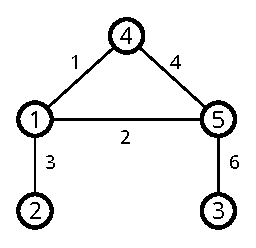
\includegraphics[scale=1.0]{random_walk}
\end{center}
\end{column}
\begin{column}{0.6\textwidth}
\[
P_{ij} = \frac{w(i,j)}{\sum_k w(i,k)}
\]
where $w(a,b)$ is the weight of edge $(a,b)$.\\
To make it as a time-reversible chain, we let
\[
\pi_i = \frac{\sum_k w(i,k)}{\sum_\ell \sum_k w(\ell,k)} \quad\forall i
\]
We can see that
\[
\pi_i\cdot P_{ij} = \pi_j\cdot P_{ji} \quad\forall i,j
\]
\end{column}
\end{columns}
\end{frame}

\begin{frame}{Hastings-Metropolis sampling algorithm}
Design an irreducible Markov chain $\mathbb{X}$ such that the unique stationary distribution of $\mathbb{X}$ is the distribution of random variable $Y$.\\
Since the long-run proportion of state $i$ is $P(Y=i)$,
\[
\lim_{n\to\infty} \frac{X(1)+X(2)+\ldots+X(n)}{n} = \sum_{i\in S} i\cdot P(Y=i) = E[Y] = \mu
\]

While computing $\mu$ by the law of large number is difficult (hard to sample on $Y$), we use this alternative method to compute $\mu$ by generating a sequence of $\mathbb{X}$, which is sometime easier.
\end{frame}

\begin{frame}{Hastings-Metropolis sampling algorithm (cont.)}\label{possible_Y}
There's a random variable $Y$ such that
\[
P(Y=i) = \frac{b_i}{C}
\]
for some unknown (or intractable) $C = \sum_{i\in S}b_i$.\\
We then design a Markov chain $\mathbb{X}$ that
\begin{itemize}
\item $P_{ii} = Q_{ii} + \sum_{k\in S, k\neq i} Q_{ik}\cdot (1-q_{ik})$
\item $P_{ij} = Q_{ij}\cdot q_{ij} \quad\forall j\neq i$
\end{itemize}
where
\begin{itemize}
\item $Q$ is the transition matrix of an arbitrary irreducible Markov chain $\mathbb{X}$ which has the same state space as $Y$.
\item $q$ is a matrix to be determined later.
\end{itemize}
\end{frame}

\begin{frame}{Hastings-Metropolis sampling algorithm (cont.)}
For $n = 0,1,\ldots$,
\begin{enumerate}
\item If $X(n)=i$, set $Z$ such that $P(Z = j) = Q_{ij} \quad\forall j\in S$.
\item If $Z = j$, set $X(n+1)$ such that
	\begin{itemize}
	\item $P(X(n+1)=j) = q_{ij}$
	\item $P(X(n+1)=i) = 1 - q_{ij}$
	\end{itemize}
\end{enumerate}
One can see that this satisfies the requirement on previous page.
\end{frame}

\begin{frame}{Hastings-Metropolis sampling algorithm (cont.)}
Then, we let
\begin{align*}
& q_{ij} = \min\left( \frac{b_j\cdot Q_{ji}}{b_i\cdot Q_{ij}}, 1 \right) \\
\implies & b_i\cdot Q_{ij}\cdot q_{ij} = b_j\cdot Q_{ji}\cdot q_{ji} \\
\implies & \frac{b_i}{C}\cdot P_{ij} = \frac{b_j}{C}\cdot P_{ji}
\end{align*}
By observation 3 on page \pageref{obs3}, we know that $(b_1/C, b_2/C,\ldots)$ is the stationary distribution of $\mathbb{X}$.
\end{frame}

\begin{frame}{Example: Space of permutations}
\begin{example}
Let $S$ consist of all the permutations $(x_1, x_2, \ldots, x_n)$ of $\{1,2,\ldots,n\}$ that
\[
\sum_{k=1}^n k\cdot x_k \geq \frac{n^3}{4}
\]
\end{example}
\begin{itemize}
\item This is same as $Y$ in page \pageref{possible_Y} with $C=|S|$ and $b_i = 1 ~\forall i$.
\item $S$ is hard to compute.
\item We need to design a matrix $Q$ such that when given a permutation $x$, it's efficient to compute the value of $Q_{xy} ~\forall y\in S$.
\end{itemize}
\end{frame}

\begin{frame}{Example: Space of permutations (cont.)}
We let
\[
Q_{xy} = \frac{1}{N(x)} \quad,\text{if $y$ can be obtained from $x$ by one swap}
\]
where $N(x)$ is the number of permutations that can be obtained from $x$ by one swap.
For example:
\[
\underbrace{(1,2,3,4,5)}_y \leftrightarrow 
\underbrace{(1,3,2,4,5)}_x \leftrightarrow 
\underbrace{(1,3,4,2,5)}_y
\]
This chain is irreducible since each $x\in S$ can go to $(x_1,x_2,\ldots,x_n)$, where $x_1 \leq x_2 \leq \ldots \leq x_n$, by several swaps.\\
Also, given a $x$, finding all the obtainable $y$ can be done efficiently.
\end{frame}

\begin{frame}{Counting process}
\begin{definition}
A collection $\mathbb{N}$ of random variables is a \emph{counting process} if $N(t)$ denotes the total number of events that occur by time $t$.
\end{definition}
\begin{itemize}
\item $N(t)$ is a nonnegative integer.
\item The value of $N(t)$ is increasing as $t$ increase.
\item $N(t) - N(s)$ is the number of events that occur between time index $s$ and $t$, where $t > s$.
\end{itemize}
\end{frame}

\begin{frame}{Two properties}
\textbf{Independent increments}:
\begin{definition}
A counting process is \emph{independent increments} if the number of events in two non-overlapping time intervals are independent.
\end{definition}
\begin{itemize}
\item For example, $N(s) - N(0)$ and $N(s+t) - N(s)$ are independent.
\end{itemize}
\textbf{Stationary increments}:
\begin{definition}
A counting process is \emph{stationary increments} if the number of events in any time interval depends only on the  length of the interval.
\end{definition}
\begin{itemize}
\item For example, $P(N(s_1 + t) - N(s_1) = k) = P(N(s_2 + t) - N(s_2) = k)$.
\end{itemize}
\end{frame}

\begin{frame}{Poisson process}
\begin{definition}
A \emph{Poisson process} with rate $\lambda$ is a counting process with independent increments and stationary increments such that
\[
P(N(s+t)-N(s) = n) = \frac{e^{-\lambda t}\cdot (\lambda t)^n}{n!}
\]
holds for all nonnegative integers.
\end{definition}
\begin{itemize}
\item $N(s+t)-N(s)$ is Poisson distributed with parameter $\lambda t$.
\item The average number of events that occur in an unit time interval ($t=1$) is $\lambda$ (since the expectation value of Poisson distribution with parameter $\lambda$ is $\lambda$.)
\end{itemize}
\end{frame}

\begin{frame}{An operational definition}\label{operation_def}
\begin{theorem}
Let $\mathbb{N}$ be a counting process with independent increments and stationary increments.
Then $\mathbb{N}$ is a Poisson process if and only if the following two conditions hold:
\begin{enumerate}
\item $P(N(t)=1) = \lambda\cdot t + o(t)$
\item $P(N(t)\geq 2) = o(t)$
\end{enumerate}
\end{theorem}
\begin{itemize}
\item We say that $f(t)=o(t)$ if
\[
\lim_{t\to 0} \frac{f(t)}{t} = 0
\]
\end{itemize}
\end{frame}

\begin{frame}{Proof}
($\Longrightarrow$):\\
Since $N(t)$ is Poisson distributed with parameter $\lambda t$,
\begin{align*}
P(N(t)=1) = \frac{(\lambda t)\cdot e^{-\lambda t}}{1!} & = \lambda t 
	\cdot\left(1 - \frac{\lambda t}{1!} + \frac{(\lambda t)^2}{2!} - \cdots\right) \\
& = \lambda t - {\lambda}^2 t^2 + \cdots \\
& = \lambda t + o(t)
\end{align*}
\begin{align*}
P(N(t)=2) = \frac{(\lambda t)^2\cdot e^{-\lambda t}}{2!} & = \frac{(\lambda t)^2}{2!}
	\cdot\left(1 - \frac{\lambda t}{1!} + \frac{(\lambda t)^2}{2!} - \cdots\right) \\
& = o(t)
\end{align*}
One can prove that $P(N(t) = k) = o(t)$ for all $k \geq 2$,\\
hence $P(N(t)\geq 2) = o(t)$.
\end{frame}

\begin{frame}{Proof (cont.)}
($\Longleftarrow$):\\
The Laplace transform of a random variable $X$ is
\[
\phi(u) = E[e^{-u\cdot X}]
\]
We say that two random variables have the same distribution if their Laplace transform are the same.\\
And if $X$ is Poisson distributed with parameter $\lambda t$, then
\[
E[e^{-u\cdot X}] = e^{(e^{-u} - 1)\cdot \lambda t}
\]
\end{frame}

\begin{frame}{Proof (cont.)}
We define $\phi_u(t) = E[e^{-u\cdot N(t)}]$, then we know that
\begin{align*}
\phi_u(s+t) & = E[e^{-u\cdot N(s+t)}] \\
& = E[e^{-u\cdot(N(s)-N(0))} e^{-u\cdot(N(s+t)-N(s))}] \\
& = E[e^{-u\cdot N(s)}]\cdot E[e^{-u\cdot (N(s+t) - N(s))}] \\
& = E[e^{-u\cdot N(s)}]\cdot E[e^{-u\cdot N(t)}] \\
& = \phi_u(s)\cdot \phi_u(t)
\end{align*}
The 3rd equation is because two independent random variables $X$ and $Y$ will make
\[
E[X\cdot Y] = E[X]\cdot E[Y]
\]
\end{frame}

\begin{frame}{Proof (cont.)}
By the two conditions in page \pageref{operation_def}, we know
\[
P(N(t) = 0) = 1 - \lambda t + o(t)
\]
Therefore,
\begin{align*}
\phi_u(t) & = E[e^{-u\cdot N(t)}] \\
& = e^{-u\cdot 0}\cdot (1 - \lambda t + o(t)) + e^{-u\cdot 1}\cdot (\lambda t + o(t)) \\
& \qquad + (e^{-u\cdot 2} + e^{-u\cdot 3} + \cdots)\cdot o(t) \\
& = 1 - \lambda t + e^{-u} \cdot \lambda t + o(t) \\
& = 1 + (e^{-u} - 1)\cdot \lambda t + o(t)
\end{align*}
And
\[
\phi_u(s+t) = \phi_u(s)\cdot \phi_u(t) = \phi_u(s)\cdot (1 + (e^{-u} - 1)\cdot \lambda t + o(t))
\]
\end{frame}

\begin{frame}{Proof (cont.)}
Differentiate on $\phi_u(s)$, we can get
\begin{align*}
{\phi_u}'(s) & = \lim_{t\to 0}\frac{\phi_u(s+t) - \phi_u(s)}{t}
 = \lim_{t\to 0}(\phi_u(s)\cdot (e^{-u} - 1)\cdot \lambda + o(t)) \\
& = \phi_u(s)\cdot (e^{-u} - 1)\cdot \lambda
\end{align*}
By $\frac{{\phi_u}'(s)}{\phi_u(s)} = (e^{-u} - 1)\cdot \lambda$, we have
\[
\ln \phi_u(s) = \int (e^{-u} - 1)\cdot \lambda \; ds = (e^{-u} - 1)\cdot \lambda s + C
\]
By $\phi_u(0) = 1$ and $\ln 1 = 0$, we know $C = 0$, hence
\[
\phi_u(s) = e^{(e^{-u} - 1)\cdot \lambda s} \quad\forall s, u
\]
which means that $N(s)$ is Poisson distributed for all $s$.
\end{frame}

\begin{frame}{Inter-arrival time}
\begin{definition}
The $k$th inter-arrival time $T_k$ of $\mathbb{N}$ is the time interval between the $(k+1)$st and $k$th events.\\
$\mathbb{T} = T_1, T_2, \ldots$ is the sequence of inter-arrival times of $\mathbb{N}$.
\end{definition}
\begin{itemize}
\item $0$th event arrives at time $0$.
\end{itemize}
\end{frame}

\begin{frame}{Observation 1: Independent \& exponential distributed}
\begin{obs}
If $\mathbb{N}$ is a Poisson process with rate $\lambda$,
then each $T_k$ is an independent exponential distribution with parameter $\lambda$.
\end{obs}
\textbf{Proof}:\\
The cumulative distribution function of $T_1$ is
\begin{align*}
F_1(s) & = P(T_1 \leq s) \\
& = 1 - P(T_1 > s) \\
& = 1 - P(N(s) = 0) \\
& = 1 - e^{-\lambda s}
\end{align*}
The 3rd equation is because $T_1 > s \iff N(s) = 0$. \\
We can observe that $T_1$ is exponential distributed.
\end{frame}

\begin{frame}{Proof (cont.)}
\begin{align*}
P(T_2 > t | T_1 = s) & = P(N(T_1+t) - N(T_1) = 0 | T_1 = s) \\
& = P(N(T_1+t) - N(T_1) = 0) \\
& = P(N(t) = 0) \\
& = e^{-\lambda t}
\end{align*}
%The 2nd equation is by independent increments.\textcolor{red}{why?} \\
The equations are derived by stationary increments.\\
\vspace{\baselineskip}
Thus, $T_2$ is also exponential distributed with parameter $\lambda$. \\
And $T_1$, $T_2$ are independent. \\
One can prove for $T_k$ with $k \geq 3$ by the same approach.
\end{frame}

\begin{frame}{Observation 2: Waiting time is gamma distributed}
\begin{obs}
The waiting time $S_k = T_1 + T_2 + \cdots + T_k$ of the $k$th event is gamma distributed with parameter $(k, \lambda)$. \textcolor{red}{check gamma distribution}
\end{obs}
\begin{itemize}
\item The probability density function is
\[
f(t) = \lambda e^{-\lambda t}\cdot \frac{(\lambda t)^{k-1}}{(k-1)!}
\]
\item It's also called Erlang distribution since $k \in \mathbb{Z}^+$.
\end{itemize}
\end{frame}

\begin{frame}{Verification}
\[
P(S_k \leq t) = P(N(t) \geq k) = \sum_{i\geq k} P(N(t) = i) = \sum_{i\geq k} \frac{(\lambda t)^i \cdot e^{-\lambda t}}{i!}
\]
So,
\begin{align*}
\frac{d P(S_k \leq t)}{dt} & = \sum_{i\geq k}\frac{\lambda\cdot(\lambda t)^{i-1}\cdot e^{-\lambda t}}{(i-1)!}
	- \sum_{i\geq k}\frac{(\lambda t)^i \cdot e^{-\lambda t} \cdot \lambda}{i!} \\
& = \frac{\lambda\cdot (\lambda t)^{k-1}\cdot e^{-\lambda t}}{(k-1)!}
\end{align*}
\end{frame}

\begin{frame}{Property 1 (Different types of events)}\label{property_1}
\begin{pty}
Let $\mathbb{N}$ be a Poisson process with rate $\lambda$, 
each event is classified as type 1 with probability $p$ or type 2 with probability $1-p$.\\
Then the arrival of type 1 and type 2 events are both Poisson processes with rate $p\cdot\lambda$ and $(1-p)\cdot\lambda$.
And the two processes are independent.
\end{pty}
\begin{itemize}
\item Let $\mathbb{N}_1$ be the process of type 1 event, 
$N_1(k)$ is the number of type 1 events that occur by time $k$. (same for $\mathbb{N}_2$)
\item $\mathbb{N}_1$ and $\mathbb{N}_2$ are said to be independent if $N_1(s_1+t_1) - N_1(s_1)$ and $N_2(s_2+t_2) - N(s_2)$ are independent for all $s_1, t_1, s_2, t_2$.
\end{itemize}
\end{frame}

\begin{frame}{Proof}
Here we prove that $\mathbb{N}_1$ is a Poisson process with rate $\lambda p$.\\
\vspace{\baselineskip}
\textbf{Stationary increments}:
\[
P(N_1(s+t) - N_1(s) = k_1 | N(s+t) - N(s) = k) = \binom{k}{k_1}\cdot p^{k_1}\cdot (1-p)^{k-k_1}
\]
Therefore,
\[
P(N_1(s+t) - N_1(s) = k_1) = \sum_{k\geq 0} \binom{k}{k_1}\cdot p^{k_1}\cdot (1-p)^{k-k_1}
	\cdot \frac{(\lambda t)^k\cdot e^{\lambda t}}{k!}
\]
which has nothing to do with $s$.
\end{frame}

\begin{frame}{Proof (cont.)}
\textbf{Independent increments}:\\
Let $(s,s+t)$ and $(u,u+v)$ be two non-overlapping time intervals,
\begin{align*}
& P(N_1(s+t)-N_1(s)=k_1, N_1(u+v)-N_1(u)=\ell_1) \\
& = \sum_{k\geq 0}\sum_{\ell\geq 0} P(N_1(s+t)-N_1(s)=k_1, N_1(u+v)-N_1(u)=\ell_1 \\
& \qquad | N(s+t)-N(s)=k, N(u+v)-N(u)=\ell) \\
& \qquad \cdot P(N(s+t)-N(s)=k, N(u+v)-N(u)=\ell) \\
& = \sum_{k\geq 0}\sum_{\ell\geq 0} P(N_1(s+t)-N_1(s)=k_1 | N(s+t)-N(s)=k) \\
& \qquad\cdot P(N_1(u+v)-N_1(u)=\ell_1 | N(u+v)-N(u)=\ell) \\
& \qquad\cdot P(N(s+t)-N(s)=k)\cdot P(N(u+v)-N(u)=\ell) \\
& = P(N_1(s+t)-N_1(s)=k_1)\cdot P(N_1(u+v)-N_1(u)=\ell_1)
\end{align*}
\end{frame}

\begin{frame}{Proof (cont.)}
\textbf{Conditions on page \pageref{operation_def}}:
\begin{align*}
\textbf{1. } P(N_1(t)\geq 2) & \leq P(N(t)\geq 2) = o(t) \\
\textbf{2. } P(N_1(t)=1) & = P(N_1(t)=1 | N(t)=1)\cdot P(N(t)=1) \\
& \qquad + P(N_1(t)=1 | N(t)\geq 2)\cdot P(N(t)\geq 2) \\
& = p\cdot (\lambda t + o(t)) + o(t) \\
& = p\lambda t + o(t)
\end{align*}
Hence we know that $\mathbb{N}_1$ is a Poisson process with rate $\lambda p$.\\
\textcolor{red}{Seems like we can also derive this from the result of next page and omit this page's proof? (By Example 3.23 on textbook?)}
\end{frame}

\begin{frame}{Proof (cont.)}
\textbf{$\mathbb{N}_1$ and $\mathbb{N}_2$ are independent}:
\begin{align*}
& P(N_1(t) = i, N_2(t) = j) \\
& = P(N_1(t) = i, N_2(t) = j | N(t) = i+j)\cdot P(N(t) = i+j) \\
& = \binom{i+j}{i}\cdot p^i\cdot (1-p)^j\cdot \frac{e^{-\lambda t}\cdot (\lambda t)^{i+j}}{(i+j)!} \\
& = \frac{e^{-\lambda pt}\cdot (\lambda pt)^i}{i!}\cdot \frac{e^{-\lambda (1-p)t}\cdot (\lambda (1-p)t)^j}{j!} \\
& = P(N_1(t)=i)\cdot P(N_2(t)=j)
\end{align*}
We only prove for two intervals that have the same length here.\\
\textcolor{red}{This also prove that $N_1(t)$ and $N_2(t)$ are Poisson distributed over $t$ (Example 3.23 on textbook).}
\end{frame}

\begin{frame}{Example 1}
$\mathbb{N}$ has rate $10$ and $p = 1/12$,
\[
P(N_1(4) = 0) = \frac{e^{-\frac{40}{12}}\cdot (\frac{40}{12})^0}{0!} = e^{-\frac{10}{3}}
\]
\end{frame}

\begin{frame}{Example 2: Type transitions}
There're $r$ classes of particles.
\begin{itemize}
\item $Y_i(k)$ is the number of class $i$ particles at time $k$.
\item The time is discrete in this case.
\item $Y_i(0)$ is Poisson distributed with parameter $\lambda_i$.
\item $P_{ij}$ is the transition probability for a class $i$ particle to class $j$.
\end{itemize}
We prove that $Y_j(n)$ is Poisson distributed with parameter $\sum_{i=1}^r P^n_{ij}\cdot \lambda_i$.
\end{frame}

\begin{frame}{Proof}
Take class $i$ for example, we consider a Poisson process $\mathbb{N}$ with rate $\lambda_i$,
where each event is classified as type $k$ with probability $P^n_{ik}$. \\
\vspace{\baselineskip}
For an arbitrary unit time interval, the number of events that occur in this interval is Poisson distributed with parameter $\lambda_i$.
We take this Poisson distributed number as the value of $Y_i(0)$. \\
\vspace{\baselineskip}
By property 1, we know that the number of type $k$ events in this interval is Poisson distributed with parameter $P^n_{ik}\cdot \lambda_i$, which also means that the number of class $i$ particles that eventually become class $k$ at time $n$, which is denoted as $C^n_{ik}$, is also Poisson distributed with parameter $P^n_{ik}\cdot \lambda_i$. \\
\vspace{\baselineskip}
$Y_j(n) = \sum_i C^n_{ij}$, which is Poisson distributed with parameter $\sum_{i=1}^r P^n_{ij}\cdot \lambda_i$. \\
(since the Poisson parameter can be summed up.)
\end{frame}

\begin{frame}{Example 3: Selling a product}
Consider a Poisson process with rate $\lambda$, where each event is an offer that has density function $f(x)$.\\
A product is sold if an offer with value higher than the price $y$ comes.\\
Assume the accepted offer comes at time $t$, then the storage cost is $c\cdot t$, where $c$ is a constant decided by the product.\\
\vspace{\baselineskip}
We want to know the expected profit, which is $E[f(x)-ct | f(x)\geq y]$.
\end{frame}

\begin{frame}{Solution}
The probability for each offer being accepted is
\[
p(y) = P(X\geq y) = \int_y^\infty f(x)\; dx
\]
The expectation of storage time $t$ is $1/(\lambda\cdot p(y))$.\\
Hence,
\begin{align*}
& E[f(x) | f(x)\geq y] - E[ct | f(x)\geq y] \\
& = \int_0^\infty x\cdot f_{X|X\geq y}(x)\; dx - \frac{c}{\lambda\cdot p(y)} \\
& = \int_y^\infty x\cdot \frac{f_X(x)}{P(X\geq y)}\; dx - \frac{c}{\lambda\cdot p(y)} \\
& = \frac{1}{p(y)}\left( \int_y^\infty x\cdot f(x)\; dx - \frac{c}{\lambda} \right)
\end{align*}
\end{frame}

\begin{frame}{Example 4: Coupon collection}
\begin{center}

\includegraphics[scale=0.2]{coupon.png}
\end{center}
There are $r$ types of coupons, and $p_i$ is the probability for a collected coupon being type $i$.\\
\vspace{\baselineskip}
We want to know the expectation of $N$, where $N$ is the number of collected coupons so that all $r$ types of coupons are collected.
\end{frame}

\begin{frame}{Solution: First attempt}
Let $N_i$ be the number of coupons collected to receive the first type $i$ coupon.
We know that
\[
E[N] = E[\max(N_1, N_2, \ldots, N_r)]
\]
And
\[
P(N\leq n) = P(N_1\leq n, N_2\leq n, \cdots, N_r\leq n)
\]
But since each $N_i$ are not independent, we can't go even further from here.\\
For example, given that $N_1 = 1$, $P(N_2 = 1|N_1 = 1) = 0$.
\end{frame}

\begin{frame}{Solution: Second attempt}
Without loss of generality, we assume that the coupons arrive as a Poisson process $\mathbb{N}$ with rate $1$.\\
$\mathbb{N}_i$ is the process of type $i$ coupons, which has rate $p_i$.\\
$X_i$ is the time that the first type $i$ coupon appears, and
\[
X = \max(X_1, X_2, \ldots, X_r)
\]
$X_1, X_2, \ldots, X_r$ are independent since $\mathbb{N}_1, \mathbb{N}_2, \ldots, \mathbb{N}_r$ are independent.
\end{frame}

\begin{frame}{Solution: Second attempt (cont.)}
We can see that
\begin{align*}
P(X\leq t) & = P(X_1\leq t, X_2\leq t, \cdots, X_r\leq t) \\
& = \prod_{i=1}^r P(X_i\leq t) = \prod_{i=1}^r (1 - e^{-t\cdot p_i})
\end{align*}
And
\[
E[X] = \int_0^\infty P(X > t)\; dt = \int_0^\infty 1 - \prod_{i=1}^r (1 - e^{-t\cdot p_i})\; dt
\]
The first equation is from the property of probability.\\
Surprisingly, $E[X] = E[N]$ as explained below.
\end{frame}

\begin{frame}{Solution: Second attempt (cont.)}
\[
X = T_1 + T_2 + \cdots + T_N
\]
where $T_j$ is the $j$th inter-arrival time of $\mathbb{N}$.\\
Each $T_j$ are i.i.d.\ and are exponential distributed with rate $1$.\\
Also, $N$ is independent with each $T_j$.
\[
E[X|N=n] = E[T_1 + T_2 + \cdots + T_n] = n\cdot E[T_1] = n
\]
\[
E[X|N] = N\cdot E[T_1] = N
\]
Hence,
\[
E[X] = E[E[X|N]] = E[N]
\]
\end{frame}

\begin{frame}{Property 2-simple (Distribution of one event)}
\begin{pty}
Given that exactly one event of a Poisson process arrives in the interval $[0,t]$,
this arrival time is uniformly distributed over $[0,t]$.
\end{pty}
\textbf{Proof}:
\begin{align*}
P(T_1\leq s | N(t)=1) & = \frac{P(T_1\leq s, N(t)=1)}{P(N(t)=1)} \\
& = \frac{P(N(s)=1)\cdot P(N(t)-N(s)=0)}{e^{-\lambda t}\cdot (\lambda t)^1 / 1!}\\
& = \frac{e^{-\lambda s}\cdot \lambda s \cdot e^{-\lambda(t-s)}}{e^{-\lambda t}\cdot \lambda t}
= \frac{s}{t}
\end{align*}
\end{frame}

\begin{frame}{Property 2-advanced (Distribution of several events)}
\begin{pty}
Given that exactly $n$ events of a Poisson process arrive in the interval $[0,t]$,
each with arrival time $X_1, X_2, \ldots, X_n$.\\
The order statistics $X_{(1)}, X_{(2)}, \ldots, X_{(n)}$ of these random variables have the joint density function
\begin{align*}
& f_{X_{(1)}, X_{(2)}, \ldots, X_{(n)}}(x_1, x_2, \ldots, x_n | N(t)=n) \\
& = \left\{
\begin{array}{l l}
\frac{n!}{t^n} & \quad\text{if } 0 < x_1 < x_2 < \cdots < x_n < t \\
0 & \quad\text{otherwise} \\
\end{array}
\right.
\end{align*}
\end{pty}
\begin{itemize}
\item This implies that $X_1, X_2, \ldots, X_n$ are i.i.d.\ and each is uniformly distributed over $[0,t]$.
\end{itemize}
\end{frame}

\begin{frame}{Proof}
For any $0 < x_1 < x_2 < \ldots < x_n < t$,
\begin{align*}
& f_{X_{(1)}, X_{(2)}, \ldots, X_{(n)}}(x_1, x_2, \ldots, x_n | N(t)=n) \\
& = \frac{f_{X_{(1)}, X_{(2)}, \ldots, X_{(n)}, N(t)}(x_1, x_2, \ldots, x_n, n)}{P(N(t) = n)} \\
& = \frac{f_{T_1, T_2, \ldots, T_n}(x_1, x_2 - x_1, \ldots, x_n - x_{n-1})\cdot P(T_{n+1} > t - x_n)}{P(N(t) = n)} \\
& = \frac{\lambda e^{-\lambda x_1}\cdot\lambda e^{-\lambda(x_2-x_1)}\cdots\lambda e^{-\lambda(x_n-x_{n-1})}\cdot e^{-\lambda(t-x_n)}}{\frac{e^{-\lambda t}(\lambda t)^n}{n!}} \\
& = \frac{n!}{t^n}
\end{align*}
$T_i$ are the inter-arrival times, which are exponential distributed.
\end{frame}

\begin{frame}{Corollary of two properties (simple version)}
\begin{corollary}
Consider a Poisson process with rate $\lambda$.\\
Each event is classified into a type $i$, where there are $r$ types of event. \\
Suppose that $p_i(\cdot)$ is a sampling function over interval $[0,t]$ such that
each arrived event at time $x$ has probability $p_i(x)$ to be classified as type $i$.\\
Then the number $N_i(t)$ of type $i$ events in $[0,t]$ is Poisson distributed with parameter
\[
\lambda \int_0^t p_i(x)\; dx = \lambda\cdot t\cdot R_i \quad\text{,where }R_i = \frac{1}{t}\int_0^t p_i(x)\; dx
\]
And each $N_i(t)$ for all $i$ are independent.
\end{corollary}
\begin{itemize}
\item $N_i(\cdot)$ does not form a Poisson process here. \\
It doesn't satisfy stationary distribution because of $p_i(\cdot)$.
\end{itemize}
\end{frame}

\begin{frame}{Proof}
Assume that $N(t)=n$. \\
Let $n = n_1 + n_2 + \cdots + n_r$, where $n_i \geq 0 ~\forall i=1,\ldots,r$.\\
These $n$ events arrive independent and uniformly at random over $[0,t]$.\\
If an event arrives at time $x \in [0,t]$, then with probability $p_i(x)$ it becomes type $i$.
Therefore, each event is of type $i$ with probability
\begin{align*}
& \int_0^t P(\text{type } i | \text{arrives at time } x)\cdot \frac{1}{t} \; dx \\
& = \frac{1}{t} \int_0^t p_i(x)\; dx \\
& = R_i
\end{align*}
which can be seen as the average of $p_i(\cdot)$ over $[0,t]$.
\end{frame}

\begin{frame}{Proof (cont.)}
\begin{align*}
P(\bigwedge_{1\leq i\leq r} N_i(t) = n_i) & = P(\bigwedge_{1\leq i\leq r} N_i(t) = n_i | N(t)=n)\cdot P(N(t)=n)\\
& = \left( \frac{n!}{n_1! n_2!\cdots n_r!}\cdot \prod_{1\leq i\leq r}{R_i}^{n_i} \right)
\cdot \frac{e^{-\lambda t}\cdot(\lambda t)^n}{n!}\\
& = \prod_{1\leq i\leq r}\frac{e^{-\lambda t R_i}(\lambda t R_i)^{n_i}}{n_i!}\\
& = \prod_{1\leq i\leq r}P(N_i(t) = n_i)
\end{align*}
Hence we know that each $N_i(t)$ is Poisson distributed with parameter $\lambda t R_i$ and are independent.
(Check Example 3.23 on textbook.)
\end{frame}

\begin{frame}{Corollary of two properties (full version)}
\begin{corollary}
Consider a Poisson process with rate $\lambda$.\\
Each event is classified into a type $i$, where there are $r$ types of event. \\
Suppose that $p_i(\cdot)$ is a sampling function over interval $[s,s+t]$ such that
each arrived event at time $x$ has probability $p_i(x)$ to be classified as type $i$.\\
Then the number $N_i(s+t)-N_i(s)$ of type $i$ events in $[s,s+t]$ is Poisson distributed with parameter
\[
\lambda \int_s^{s+t} p_i(x)\;dx
\]
And each $N_i(s+t)-N_i(s)$ for all $i$ are independent.
\end{corollary}
\end{frame}

\begin{frame}{Proof}
Regarding $[s, s+t]$ as $[0,t]$, the sampling function becomes
\[
p'_i(x) = p_i(x+s)
\]
From the simple version, we know that $N_i(s+t)-N_i(s)$ is Poisson distributed with parameter
\[
\lambda\int_0^t p'_i(x)\;dx = \lambda\int_0^t p_i(x+s)\;dx = \lambda\int_s^{s+t} p_i(x)\;dx
\]
\end{frame}

\begin{frame}{Example 1: Infinite server queue}
\begin{center}

\includegraphics[scale=0.13]{server.png}
\end{center}
Suppose that jobs arrive at a Poisson rate $\lambda$, and we have infinite number of servers.
The running time of each job is independent and distributed with function $T(\cdot)$.
We want to know
\begin{enumerate}
\item The distribution of the number $X(t)$ of completed jobs by time $t$.
\item The distribution of the number $Y(t)$ of running jobs by time $t$.
\item The joint distribtuion of $Y(t_1)$ and $Y(t_2)$, where $t_1 < t_2$.
\end{enumerate}
\end{frame}

\begin{frame}{Solution of question 1 \& 2}
We classify the jobs into two types:
\begin{itemize}
\item \textbf{type 1}: completed by time $t$.
\item \textbf{type 2}: not completed by time $t$.
\end{itemize}
If a job arrives at time $x$, then the sampling function is
\begin{itemize}
\item $p_1(x) = T(t-x)$
\item $p_2(x) = 1 - T(t-x)$
\end{itemize}
Thus, $X(t) = N_1(t)$ is Poisson distributed with parameter
\[
\lambda\int_0^t T(t-x)\;dx
\]
And $Y(t) = N_2(t)$ is Poisson distributed with parameter
\[
\lambda\int_0^t (1-T(t-x))\;dx = \lambda t - \lambda\int_0^t T(t-x)\;dx
\]
\end{frame}

\begin{frame}{Solution of question 3}
\begin{center}
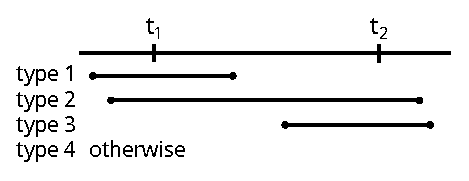
\includegraphics[scale=1.0]{infinite_server}
\end{center}
\begin{align*}
p_1(x) & = T(t_2-x) - T(t_1-x) \quad\text{if } 0 < x < t_1 \\
p_2(x) & = 1 - T(t_2-x) \quad\text{if } 0 < x < t_1 \\
p_3(x) & = 1 - T(t_2-x) \quad\text{if } t_1 < x < t_2
\end{align*}
\end{frame}

\begin{frame}{Solution of question 3 (cont.)}
We know that $Y(t_1) = N_1(t_2) + N_2(t_2)$ and $Y(t_2) = N_2(t_2) + N_3(t_2)$, \\
hence $Y(t_1)$ and $Y(t_2)$ are not independent.
Therefore, we use the following method:
\begin{align*}
& P(Y(t_1) = m_1, Y(t_2) = m_2) \\
& = \sum_{n_2 = 0}^\infty P(N_1(t_2) = m_1-n_2, N_2(t_2) = n_2, N_3(t_2) = m_2-n_2) \\
& = \sum_{n_2 = 0}^\infty P(N_1(t_2) = m_1-n_2)\cdot P(N_2(t_2) = n_2)\cdot P(N_3(t_2) = m_2-n_2) \\
& = \cdots
\end{align*}
The $\infty$ in $\sum$ can be replaced by $\min(m_1, m_2)$.
\end{frame}

\begin{frame}{Example 2: Encounters on a highway}
\begin{center}
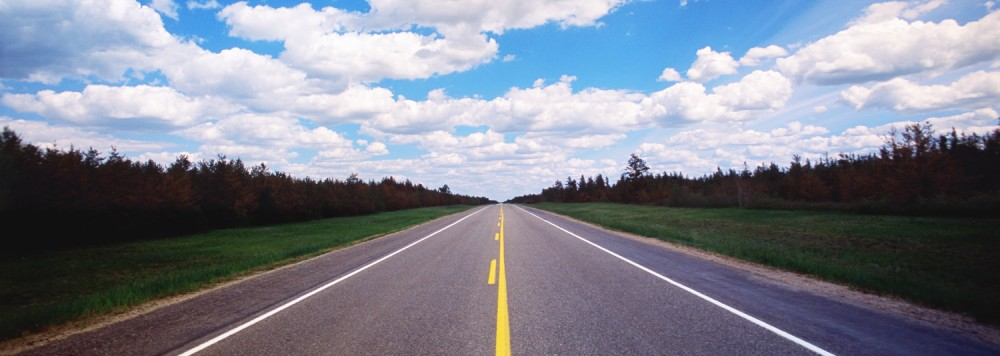
\includegraphics[scale=1]{highway_scale.jpg}
\end{center}
Cars enter a distance-$d$ highway in a Poisson rate $\lambda$.\\
The fixed speed of each car is i.i.d.\ with function $F_S(\cdot)$.\\
Suppose our car enters the highway and moves at a fixed speed $s$,
what's the distribution of the number of encountering with other cars?
\end{frame}

\begin{frame}{Solution}
Suppose we enter at time $t_1$ and leave at $t_2 = t_1 + d/s$.\\
Each car choose a fixed speed $S$ according to $F_S$, its travel time $T = d/S$.\\
The distribution function of $T$ is
\[
F_T(t) = P(T\leq t) = P(S\geq \frac{d}{t}) = 1 - F_S(\frac{d}{t})
\]
We classify the cars into three types:
\begin{itemize}
\item \textbf{type a} (overtaken by us): $0 < t < t_1$, $t + T > t_2$.
\item \textbf{type b} (overtake us): $t_1 < t < t_2$, $t + T < t_2$.
\item \textbf{type c}: otherwise
\end{itemize}
\end{frame}

\begin{frame}{Solution (cont.)}
\begin{align*}
p_a(t) & = P(T > t_2 - t) = 1 - F_T(t_2 - t) \quad\text{if } 0 < t < t_1 \\
p_b(t) & = P(T < t_2 - t) = F_T(t_2 - t) \quad\text{if } t_1 < t < t_2
\end{align*}
Since the Poisson parameters can be summed up, $N_a(t_2) + N_b(t_2)$ is Poisson distributed with parameter
\[
\lambda\int_0^{t_1} (1 - F_T(t_2 - t))\;dt + \lambda\int_{t_1}^{t_2} F_T(t_2 - t)\;dt
\]
which is the distribution we want.
\end{frame}

\begin{frame}{Example 3: HIV infection}
\begin{center}

\includegraphics[scale=0.25]{hiv.jpg}
\end{center}
People are infected with an unknown Poisson rate $\lambda$.\\
The incubation time for each infected person has distribution function $F$.\\
At time $t$, we know the number $n_1$ of people who already have the AIDS symptoms (finished incubations).\\
We want to estimate the value of $\lambda$, and the number $n_2$ of the incubating people at time $t$.
\end{frame}

\begin{frame}{Solution}
We classify the infected people into two types:
\begin{itemize}
\item \textbf{type 1}: have symptoms appear by time $t$.
\item \textbf{type 2}: still in incubation by time $t$.
\end{itemize}
Then
\begin{align*}
E[N_1(t)] & = \lambda\int_0^t F(t-x)\;dx = \lambda\int_0^t F(x)\;dx \\
E[N_2(t)] & = \lambda\int_0^t (1-F(t-x))\;dx = \lambda\int_0^t (1-F(x))\;dx \\
n_1 & \approx E[N_1(t)] \implies \hat{\lambda} = \frac{n_1}{\int_0^t F(x)\;dx} \\
n_2 & \approx \hat{\lambda}\int_0^t (1-F(x))\;dx = \frac{n_1\int_0^t (1-F(x))\;dx}{\int_0^t F(x)\;dx}
\end{align*}
\end{frame}

\begin{frame}{Example 4: Hidden bugs}
\begin{center}

\includegraphics[scale=0.3]{bug.png}
\end{center}
Suppose the errors come as a Poisson process.\\
Each error belongs to one of the $m$ bugs in the program.\\
For all $i = 1,\ldots, m$, $\mathbb{N}_i$ denotes the Poisson process of errors caused by bug $i$, which has an unknown rate $\lambda_i$.\\
At time $t$, we know the value of $M_j(t)$, which is the number of bugs causing exactly $j$ errors.\\
And a bug is still \textit{hidden} if it hasn't cause any error.\\
We want to know the expected error rate of hidden bugs, 
which is the expectation of the summation of all hidden bugs' $\lambda_i$.
\end{frame}

\begin{frame}{Solution}
Let
\begin{align*}
H_i(t) & = \left\{
\begin{array}{l l}
1 & \quad\text{if the $i$th bug is still hidden by time $t$} \\
0 & \quad\text{otherwise} \\
\end{array}
\right. \\
\Lambda(t) & = \sum_{i=1}^m H_i(t)\cdot \lambda_i
\end{align*}
Then
\begin{align*}
& P(H_i(t)=1) = P(N_i(t)=0) = \frac{(\lambda_i t)^0 \cdot e^{-\lambda_i t}}{0!} = e^{-\lambda_i t} \\
& E[\Lambda(t)] = \sum_{i=1}^m \lambda_i\cdot E[H_i(t)]
	= \sum_{i=1}^m \lambda_i\cdot P(H_i(t) = 1) = \sum_{i=1}^m \lambda_i\cdot e^{-\lambda_i t} \\
&\qquad = \frac{1}{t}\sum_{i=1}^m \lambda_i\cdot t\cdot e^{-\lambda_i t} = \frac{1}{t}\sum_{i=1}^m P(N_i(t) = 1)
	= \frac{1}{t} E[M_1(t)]
\end{align*}
\end{frame}

\begin{frame}{Non-homogeneous Poisson process}
\begin{definition}
$\mathbb{N}$ is a non-homogeneous Poisson process with intensity function $\lambda(\cdot)$ if
$\mathbb{N}$ is a counting process such that the following four conditions hold:
\begin{enumerate}
\item $N(0) = 0$
\item $\mathbb{N}$ satisfies independent increments.
\item $P(N(t+h)-N(t) \geq 2) = o(h)$
\item $P(N(t+h)-N(t) = 1) = \lambda(t)\cdot h + o(h)$
\end{enumerate}
\end{definition}
\begin{itemize}
\item It's a Poisson process without stationary increments.
\item If $\lambda(t) = \lambda$, it becomes the homogeneous (normal) Poisson process.
\end{itemize}
\end{frame}

\begin{frame}{Proposition 1}
\textbf{Part 1}:\\
For a Poisson process $\mathbb{N}$ with rate $\lambda$,
suppose that each arrived event has sampling function $p_i(t)$,
then the counting process $\mathbb{N}_i$ describing the arrival of type-$i$ events
is a non-homogeneous Poisson process with intensity function 
\[
\lambda_i(t) = \lambda\cdot p_i(t)
\]
\textbf{Part 2}:\\
All non-homogeneous Poisson process with bounded $\lambda(\cdot)$ can be obtained in the above way.\\
\textbf{Proof of part 2}: 
Since there's a $\lambda$ that $\lambda(t)\leq \lambda$ for all $t$, 
we just let $p_i(t) = \lambda(t) / \lambda$ for a Poisson process with rate $\lambda$.
\end{frame}

\begin{frame}{Proof of part 1}
\textbf{Condition 1}: trivial.\\
\textbf{Condition 3}:
\[
P(N_i(t+h)-N_i(t)\geq 2)\leq P(N(t+h)-N(t)\geq 2) = o(h)
\]
\textbf{Condition 4}:
\begin{align*}
& P(N_i(t+h)-N_i(t) = 1) \\
= & \colorbox{yellow}{$P(N_i(t+h)-N_i(t) = 1 | N(t+h)-N(t) = 1)$} \\
& \qquad \times \colorbox{green}{$P(N(t+h)-N(t) = 1)$} \\
& \qquad + P(N_i(t+h)-N_i(t) = 1 | N(t+h)-N(t)\geq 2) \\
& \qquad \times \colorbox{cyan}{$P(N(t+h)-N(t)\geq 2)$} \\
= & \colorbox{yellow}{$(p_i(t) + o(h))$}\cdot \colorbox{green}{$(\lambda h + o(h))$} + \colorbox{cyan}{$o(h)$} \\
= & p_i(t)\cdot \lambda h + o(h)
\end{align*}
\end{frame}

\begin{frame}{Proof of part 1 (cont.)}
The \colorbox{yellow}{yellow} part holds because
\begin{align*}
& \lim_{h\to 0} P(N_i(t+h)-N_i(t) = 1 | N(t+h)-N(t) = 1) = p_i(t) \\
\implies & P(N_i(t+h)-N_i(t) = 1 | N(t+h)-N(t) = 1) = p_i(t) + o(h)
\end{align*}
\textbf{Condition 2}:\\
Consider non-overlapped intervals $[s,s+t]$ and $[u,u+v]$, 
the distribution in each interval is decided by Poisson parameter $\lambda\int_s^{s+t} p_i(x)\;dx$ and $\lambda\int_u^{u+v} p_i(x)\;dx$, which doesn't influence each other.
\end{frame}

\begin{frame}{Distribution of non-homogeneous Poisson process}
According to part 2 of proposition 1, 
for a non-homogeneous Poisson process with intensity function $\lambda(\cdot)$,
we can observe that its distribution in $[s,s+t]$ is Poisson distributed with parameter
\[
\lambda\int_s^{s+t} p_i(x)\;dx = \int_s^{s+t} \lambda(x)\;dx
\]
\end{frame}

\begin{frame}{Example 1: Poisson tea shop}
Suppose that customers come to tea shop as a non-homogeneous Poisson process with $\lambda(t)$ as follow:
\[
\lambda(t) = \left\{
\begin{array}{l l}
0 & 0\leq t\leq 8 \\
5 + 5\cdot(t-8) & 8 < t\leq 11 \\
20 & 11 < t < 13 \\
20 - 2\cdot(t-13) & 13 < t\leq 17 \\
0 & 17 < t < 24 \\
\end{array}
\right.
\]
We want to know the probability that no one comes in $[8.5,9.5]$.
\end{frame}

\begin{frame}{Solution}
The distribution in $[8.5,9.5]$ is a Poisson with parameter
\[
\int_{8.5}^{9.5} (5+5\cdot(t-8))\;dt = \int_{0.5}^{1.5} (5+5t)\;dt = 10
\]
Hence the probability is $e^{-10}$.
\end{frame}

\begin{frame}{Example 2: Infinite server queue again}
\begin{center}

\includegraphics[scale=0.13]{server.png}
\end{center}
Suppose that jobs arrive at a Poisson rate $\lambda$, and we have infinite number of servers.
The running time of each job is independent and distributed with function $F(\cdot)$.\\
We want to prove that the process of jobs departing (finishing) is a non-homogeneous Poisson process.
\end{frame}

\begin{frame}{Proof}
\textbf{Condition 1}: trivial.\\
\vspace{\baselineskip}
\textbf{Condition 2}:\\
Consider two non-overlapping intervals $[s,s+t]$ and $[u,u+v]$, where $u > s$.
Let the jobs finishing in $[s,s+t]$ be type 1, and those finishing in $[u,u+v]$ be type 2.\\
According to corollary of property 2, we know that the distribution of type 1 and type 2 jobs are independent in $[0,u+v]$, which means that the number of jobs finishing in $[s,s+t]$ and $[u,u+v]$ are independent.
\end{frame}

\begin{frame}{Proof (cont.)}
\textbf{Condition 3 \& 4}:
Let $f(\cdot)$ be the density function of $F(\cdot)$.
The number of jobs departing in $[t,t+h]$ is Poisson distributed with parameter
\begin{align*}
& \lambda\int_0^{t+h}(F(t+h-x)-F(t-x))\;dx \\
= & \lambda\int_0^{t+h}(f(t+h-x)\cdot h + o(h))\;dx \\
= & \left( \lambda h \int_0^{t+h} f(x)\;dx \right) + o(h) \\
= & \lambda h\cdot F(t+h) + o(h) \\
= & \lambda h\cdot F(t) + o(h)
\end{align*}
\end{frame}

\begin{frame}{Proof (cont.)}
The first equation is because
\[
\lim_{h\to 0}\frac{F(t+h-x)-F(t-x)}{h} = f(t-x) = \lim_{h\to 0}f(t-x+h)
\]
Then we know that
\begin{align*}
& P(N(t+h)-N(t) = 1) \\
= & (\lambda h\cdot F(t) + o(h))\cdot e^{-\lambda h\cdot F(t) + o(h)} \\
= & (\lambda h\cdot F(t) + o(h))\cdot (1 - \lambda h\cdot F(t) + o(h)) \\
= & \lambda h\cdot F(t) + o(h) \\
\text{and}\qquad & P(N(t+h)-N(t)\geq 2) \\
= & \sum_{k\geq 2}\frac{(\lambda h\cdot F(t) + o(h))^k \cdot e^{-\lambda h\cdot F(t) + o(h)}}{k!} \\
= & o(h)
\end{align*}
\end{frame}

\begin{frame}{Proposition 2}
If $\mathbb{N}_1$ and $\mathbb{N}_2$ are independent non-homogeneous Poisson process with intensity function $\lambda_1(\cdot)$ and $\lambda_2(\cdot)$, \\
then $\mathbb{N} = \mathbb{N}_1 + \mathbb{N}_2$ is also a non-homogeneous Poisson process with intensity function $\lambda(t) = \lambda_1(t) + \lambda_2(t)$.\\
\vspace{\baselineskip}
\textbf{Proof} is left as exercise. (Proposition 5.4 in textbook)
\end{frame}

\begin{frame}{Continuous Markov chain}
\begin{definition}
The collection $\mathbb{X} = \{X(t) | t\geq 0\}$ of nonnegative integral random variables is a \emph{continuous-time Markov chain} if for all function $x(\cdot)$, nonnegative real numbers $s$ and $t$, and integer $i$ and $j$,
\begin{align*}
& P(X(s+t) = j | X(s) = i, X(r) = x(r) \quad\forall r \in [0,s)) \\
= & P(X(s+t) = j | X(s) = i)
\end{align*}
holds.
\end{definition}
\begin{itemize}
\item The condition above is called \emph{Markovian property}.
\item Non-homogeneous Poisson process is a continuous Markov chain, where we take the values of $N(t)$ as the states.
\end{itemize}
\end{frame}

\begin{frame}{Homogeneous transition probabilities}
\begin{definition}
We say a continuous Markov chain has homogeneous transition probabilities if 
\[
P(X(s+t) = j | X(s) = i)
\]
is independent of $s$.
\end{definition}
\begin{itemize}
\item Our discussion of continuous Markov chain assumes this property.
\end{itemize}
\end{frame}

\begin{frame}{State graph}
\begin{center}
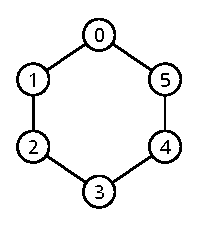
\includegraphics[scale=1.0]{state_graph}
\end{center}
The state graph of continuous Markov chain can be taken as the state graph of Markov chain without self-links.
The process will stay on a state for a certain amount of time, and go into a possible next state.
\end{frame}

\begin{frame}{Observation 1}
\begin{obs}
The time for $\mathbb{X}$ to stay in state $i$ is exponentially distributed.
\end{obs}
\begin{itemize}
\item Suppose that $X(r) = i$ for some time $r\geq 0$.
Let $T_i$ be the waiting time for $\mathbb{X}$ to transit to a state other than $i$.
We want to prove that $T_i$ is memoryless, that is
\[
P(T_i\geq s+t | T_i\geq s) = P(T_i\geq t)
\]
hence $T_i$ is exponential distributed.
\item This also means that for a Poisson process, no matter when the last event happened before, start measuring from now, the waiting time for the next event is still exponential distributed with parameter $\lambda$.
\end{itemize}
\end{frame}

\begin{frame}{Proof}
\begin{align*}
& P(T_i\geq s+t | T_i\geq s) \\
= & P(X(v)=i, \forall r+s\leq v\leq r+s+t | X(u)=i, \forall r\leq u\leq r+s) \\
\colorbox{cyan}{=} & P(X(v)=i, \forall r+s\leq v\leq r+s+t | X(r+s)=i) \\
\colorbox{yellow}{=} & P(X(v)=i, \forall r\leq v\leq r+t | X(r)=i) \\
= & P(T_i\geq t)
\end{align*}
\colorbox{yellow}{=} holds because of homogeneous transition probability. \\
\colorbox{cyan}{=} holds because of Markovian property (more details at next page.)
\end{frame}

\begin{frame}{Proof (cont.)}
\colorbox{cyan}{=} \textcolor{red}{holds because we can use something like}
\begin{align*}
& P(A, B, C, \ldots, Y | Z) \\
= & P(B, C, \ldots, Y | A, Z)\cdot P(A | Z) \\
= & P(C, \ldots, Y | A, B, Z)\cdot P(B | A, Z)\cdot P(A | Z) \\
= & \cdots
\end{align*}
\textcolor{red}{and rearrange the condition parts?}
\end{frame}

\begin{frame}{Observation 2}
\begin{obs}
Given that $X(s)=i$, the probability that the next state other than $i$ is $j$ is a value $\mathbb{P}[i,j]$ that is independent of $s$.
\end{obs}
\textbf{Proof}: For any state $j$ other than $i$, let $T_i$ be the waiting time for the first transition from state $i$ to a state other than $i$.
We have
\[
\mathbb{P}[i,j] = P(X(T_i + s) = j | X(s) = i) = P(X(T_i) = j | X(0) = i)
\]
where the last equation is by homogeneous transition probability.
\end{frame}

\begin{frame}{Interpretation}
\begin{itemize}
\item Starting with $X(0) = i$, the time staying in $i$ is exponential distributed with parameter $\lambda_i$, then $\mathbb{X}$ transits to a different state $j$ with probability $\mathbb{P}[i,j]$.
\item $\mathbb{X}$ can be characterized by
\[
\lambda_i\quad\forall i\in S \qquad\text{and}\qquad \mathbb{P}[i,j]\quad\forall i,j \in S
\]
\end{itemize}
\end{frame}

\begin{frame}{Example: Hair cut}
\begin{itemize}
\item State 0: no customer
\item State 1: cut hair
\item State 2: wash hair
\end{itemize}
Assume customers appear as a Poisson process with rate $\lambda'$.
When a customer appear, if the service is in state 1 or 2, then the customer just leave.
\begin{itemize}
\item Staying time in state 1 is exponential distributed with parameter ${\lambda_1}'$.
\item Staying time in state 2 is exponential distributed with parameter ${\lambda_2}'$.
\end{itemize}
\end{frame}

\begin{frame}{Example: Hair cut (cont.)}
Characterized as follow:
\[
\mathbb{P} = 
\begin{pmatrix}
& 1 & 0 \\
0 & & 1 \\
1 & 0 & \\
\end{pmatrix}
\]
\[
\lambda_0 = \lambda', \qquad \lambda_1 = {\lambda_1}', \qquad \lambda_2 = {\lambda_2}'
\]
\end{frame}

\begin{frame}{Birth and death process}
\begin{definition}
A \emph{birth and death process} with birth rate $\{\beta_n\}, \forall n\geq 0$ and death rate $\{\delta_n\}, \forall n\geq 0$ is a Markov chain that when the state is $n$, 
\begin{itemize}
\item The waiting time $B_n$ for it to go to state $n+1$ is exponential distributed with parameter $\beta_n$.
\item The waiting time $D_n$ for it to go to state $n-1$ is exponential distributed with parameter $\delta_n$.
\end{itemize}
\end{definition}
\end{frame}

\begin{frame}{Birth and death process: characterize}
\begin{itemize}
\item $\lambda_0 = \beta_0$
\item $\lambda_n = \beta_n + \delta_n \quad\forall n > 0$
\end{itemize}
The last equation can be seen as a Poisson process with rate $\lambda_n$, where there're two types of events, one is birth and one is death.
By page \pageref{property_1}, we get the above result and
\begin{itemize}
\item $\mathbb{P}[n,n+1] = \frac{\beta_n}{\beta_n + \delta_n} \quad\forall n > 0$
\item $\mathbb{P}[n,n-1] = \frac{\delta_n}{\beta_n + \delta_n} \quad\forall n > 0$
\end{itemize}
\end{frame}

\begin{frame}{Example: M/M/s Servers}
Given $s$ servers, where
\begin{itemize}
\item Jobs arrive in a Poisson process with rate $\lambda$.
\item Processing time for each job is exponential distributed with parameter $\mu$.
\end{itemize}
The number of jobs currently waiting or processing is a B \& D process with
\begin{itemize}
\item $\beta_n = \lambda$
\item $\displaystyle{\delta_n = \left\{
\begin{array}{l l}
\mu\cdot n \quad\forall n\leq s \\
\mu\cdot s \quad\forall n > s \\
\end{array}
\right.}$
\end{itemize}
\end{frame}

\begin{frame}{Example: Linear growth with immigration}
\begin{itemize}
\item $\beta_n = \beta\cdot n + \theta$
\item $\delta_n = \delta\cdot n$
\end{itemize}
We want to know the value of $E[X(t)]$.\\
\vspace{\baselineskip}
\textbf{Solution}:
\begin{align*}
& P(X(t+h)=n+1|X(t)=n) = (\beta n + \theta)\cdot h + o(h) \quad\forall n\geq 0 \\
& P(X(t+h)=n-1|X(t)=n) = \delta n \cdot h + o(h) \quad\forall n\geq 1 \\
& P(X(t+h)=n|X(t)=n) = 1 - (\beta n + \delta n + \theta)\cdot h + o(h) \quad\forall n\geq 0
\end{align*}
Since we make $h$ close to $0$, we ignore other probability that are all $o(h)$.
\end{frame}

\begin{frame}{Solution (cont.)}
\begin{align*}
E[X(t+h)|X(t) = n] & = (n+1)\cdot ((\beta n + \theta)\cdot h + o(h)) \\
& \qquad + (n-1)\cdot (\delta n\cdot h + o(h)) \\
& \qquad + n\cdot (1-(\beta n + \delta n + \theta)\cdot h + o(h)) \\
& \qquad + o(h) \\
& \vdots \\
& = n + ((\beta - \delta)n + \theta)\cdot h + o(h)
\end{align*}
Hence,
\begin{align*}
E[X(t+h)] & = E[E[X(t+h)|X(t)]] \\
& = (1+(\beta - \delta)\cdot h)\cdot E[X(t)] + \theta h + o(h)
\end{align*}
\end{frame}

\begin{frame}{Solution (cont.)}
\begin{align*}
\frac{E[X(t+h)]-E[X(t)]}{h} & = (\beta-\delta)\cdot E[X(t)] + \theta + \frac{o(h)}{h} \\
\frac{d}{dt}E[X(t)] & = (\beta-\delta)\cdot E[X(t)] + \theta
\end{align*}
If $\beta = \delta$,
\begin{align*}
& \frac{d E[X(t)]}{dt} = \theta \\
\implies & E[X(t)] = X(0) + \theta t
\end{align*}
\end{frame}

\begin{frame}{Solution (cont.)}
If $\beta \neq \delta$, define $g(t) = (\beta-\delta)\cdot E[X(t)] + \theta$,
\begin{align*}
& g'(t) = (\beta - \delta)\cdot \frac{d}{dt}E[X(t)] = (\beta - \delta)\cdot g(t) \\
& \qquad\vdots \\
\implies & E[X(t)] = X(0)\cdot e^{(\beta - \delta) t} + \frac{\theta}{\beta - \delta}\cdot (e^{(\beta - \delta) t} - 1)
\end{align*}
Note that if $\delta > \beta$,
\[
\lim_{t\to\infty} E[t] = \frac{\theta}{\delta - \beta}
\]
which is dominated by the immigration.
\end{frame}

\begin{frame}{Increment time}
\begin{definition}
Given a birth and death process, if $X(0)=i$, the increment time is $T_i = \min\{t | X(t) = i+1\}$.
\end{definition}
\begin{itemize}
\item We want to know the value of $E[T_i]$.
\end{itemize}
\end{frame}

\begin{frame}{Expectation of increment time}
\begin{itemize}
\item If $i = 0$, $\displaystyle{E[T_0] = \frac{1}{\beta_0}}$
\item If $i > 0$,
\begin{align*}
E[T_i] & = \text{ waiting time for the first event} \\
& \qquad + 0 \cdot P(\text{the first event is birth}) \\
& \qquad + (E[T_{i-1}] + E[T_i])\cdot P(\text{the first event is death}) \\
& = \frac{1}{\beta_i + \delta_i} + 0 + (E[T_{i-1}] + E[T_i])\cdot \frac{\delta_i}{\beta_i + \delta_i} \\
\implies E[T_i] & = \frac{1}{\beta_i}\cdot (\delta_i\cdot E[T_{i-1}] + 1)
\end{align*}
\end{itemize}
\end{frame}

\begin{frame}{Transition probability function}
\begin{definition}
The \emph{transition probability function} $P_{ij}(t) = P(X(t) = j | X(0) = i)$.
\end{definition}
\begin{itemize}
\item Note that this is different from the $\mathbb{P}[i,j]$ mentioned before.
\item There's also value for $P_{ii}(t)$.
\end{itemize}
\end{frame}

\begin{frame}{Transition probability function of pure birth process}\label{pure_birth}
\begin{theorem}
If $\mathbb{X}$ is a \emph{pure birth process}, where $\delta_n = 0 \quad\forall n\geq 0$, 
and $\beta_i\neq \beta_j \quad\forall i\neq j$, then
\[
P_{ij}(t) = \left\{
\begin{array}{l l}
e^{-\beta_i t} & \quad\text{if } i = j \\
F(i,j) - F(i,j-1) & \quad\text{if } i < j \\
\end{array}
\right.
\]
where
\[
F(i,j) = P(X(t)\leq j | X(0) = i) = \sum_{i\leq k\leq j} e^{-\beta_k t} 
\prod_{i\leq r\leq j,~ r\neq k}\frac{\beta_r}{\beta_r - \beta_k}
\]
\end{theorem}
\end{frame}

\begin{frame}{Proof}
When $i < j$,
\begin{align*}
F(i,j) & = P(X(t) < j+1 | X(0) = i) \\
& = P(T_i + T_{i+1} + \cdots + T_j > t) \\
& \colorbox{yellow}{=} \sum_{i\leq k\leq j} e^{-\beta_k t} 
\prod_{i\leq r\leq j,~ r\neq k}\frac{\beta_r}{\beta_r - \beta_k}
\end{align*}
$\colorbox{yellow}{=}$ is from equation 5.6 on textbook.\\
\[
P(T_i + T_{i+1} + \cdots + T_j > t) = 1 - P(T_i + T_{i+1} + \cdots + T_j \leq t)
\]
where $P(T_i + T_{i+1} + \cdots + T_j \leq t)$ is the distribution of sum of $j-i+1$ exponential distributions where each one must has different rate.
\end{frame}

\begin{frame}{Yule process}
\begin{definition}
Yule process is a pure birth process with linear rate, 
where $\delta_n = 0~\forall n\geq 0$ and $\beta_n = \beta\cdot n~\forall n\geq 0$.
\end{definition}
According to page \pageref{pure_birth},
\[
P_{ij}(t) = \cdots = \binom{j-1}{i-1} (e^{-\beta t})^i \cdot (1 - e^{-\beta t})^{j-i} \quad\forall 1\leq i\leq j
\]
which is a negative binomial distribution with parameter $(i, e^{-\beta t})$.
\end{frame}

\begin{frame}{Instantaneous transition rate}
\begin{definition}
Given a continuous Markov chain with each state $i$ having the exponential parameter $\lambda_i$,
the \emph{instantaneous transition rate} is
\[
q_{ij} = \lambda_i\cdot \mathbb{P}[i,j]
\]
we let $q_{ii} = 0$ for the ease of later explanation.
\end{definition}
\begin{itemize}
\item Given all the $q_{ij}$, one can compute $\lambda_i$ by $\sum_{j\in S} q_{ij}$, and then compute all the value of $\mathbb{P}[i,j]$.
Hence $q_{ij}$ also characterize the continuous Markov chain.
\end{itemize}
\end{frame}

\begin{frame}{Komolgorov forward equation}
\begin{theorem}
For most of the continuous Markov chain (ex.\ birth and death process), the following holds:
\[
{P_{ij}}'(t) = \sum_{k\in S} P_{ik}(t)\cdot q_{kj} - \lambda_j\cdot P_{ij}(t)
\]
\end{theorem}
\end{frame}

\begin{frame}{Komolgorov backward equation}
\begin{theorem}
For all the continuous Markov chain, the following holds:
\[
{P_{ij}}'(t) = \sum_{k\in S} q_{ik}\cdot P_{kj}(t) - \lambda_i\cdot P_{ij}(t)
\]
\end{theorem}
\begin{itemize}
\item We only prove this equation (at page \pageref{backward_pf}).
\end{itemize}
\end{frame}

\begin{frame}{Lemma 1}
\begin{lemma}
\begin{enumerate}
\item $\displaystyle{\lim_{h\to 0}\frac{1-P_{ii}(h)}{h} = \lambda_i}$
\item $\displaystyle{\lim_{h\to 0}\frac{P_{ij}(h)}{h} = q_{ij} \quad\text{if } i\neq j}$
\end{enumerate}
\end{lemma}
We prove this lemma by proving the equivalence that
\begin{enumerate}
\item $1 - P_{ii}(h) = \lambda_i\cdot h + o(h)$
\item $P_{ij}(h) = q_{ij}\cdot h + o(h)$
\end{enumerate}
\end{frame}

\begin{frame}{Proof}
\textbf{Equation 1}: In the interval of $h$,
\begin{align*}
P_{ii}(h) & = P(\text{no transition happen}) \\
\qquad & + P(\text{more than one transitions and come back to state $i$}) \\
\implies 1 - P_{ii}(h) & = P(\text{one transition happens}) \\
\qquad & + P(\text{more than one transitions and doesn't come back}) \\
& \colorbox{yellow}{=} \lambda_i\cdot h + o(h)
\end{align*}
$\colorbox{yellow}{=}$ is according to operational definition on page \pageref{operation_def}.
\end{frame}

\begin{frame}{Proof (cont.)}
\textbf{Equation 2}: In the interval of $h$,
\begin{align*}
P_{ij}(h) & = P(\text{one $i\to j$ transition happens}) \\
\qquad & + P(\text{more than one transitions and the final state is $j$}) \\
& = (\lambda_i\cdot h + o(h))\cdot \mathbb{P}[i,j] + o(h) \\
& = \lambda_i\cdot \mathbb{P}[i,j]\cdot h + o(h) \\
& = q_{ij}\cdot h + o(h)
\end{align*}
\end{frame}

\begin{frame}{Lemma 2}
\begin{lemma}
\[
P_{ij}(t+s) = \sum_{k\in S} P_{ik}(t)\cdot P_{kj}(s) \quad\forall s\geq 0, t\geq 0
\]
\end{lemma}
\end{frame}

\begin{frame}{Proof}
\begin{align*}
P_{ij}(t+s) & = P(X(t+s) = j | X(0) = i) \\
& = \sum_{k\in S} P(X(t+s) = j, X(t) = k | X(0) = i) \\
& = \sum_{k\in S} P(X(t+s) = j | X(t) = k, X(0) = i)\cdot P(X(t) = k | X(0) = i) \\
& \colorbox{yellow}{=} \sum_{k\in S} P(X(t+s) = j | X(t) = k)\cdot P(X(t) = k | X(0) = i) \\
& \colorbox{cyan}{=} \sum_{k\in S} P(X(s) = j | X(0) = k)\cdot P(X(t) = k | X(0) = i) \\
& = \sum_{k\in S} P_{ik}(t)\cdot P_{kj}(s)
\end{align*}
$\colorbox{yellow}{=}$ is by Markovian property.\\
$\colorbox{cyan}{=}$ is by homogeneous transition probability.
\end{frame}

\begin{frame}{Proof of backward equation}\label{backward_pf}
\begin{align*}
P_{ij}(h+t) - P_{ij}(t) & \colorbox{yellow}{=} \left( \sum_{k\geq 0} P_{ik}(h)\cdot P_{kj}(t) \right) - P_{ij}(t) \\
& = \left( \sum_{k\geq 0, k\neq i} P_{ik}(h)\cdot P_{kj}(t) \right) - (1 - P_{ii}(h))\cdot P_{ij}(t) \\
\implies {P_{ij}}'(t) & = \lim_{h\to 0}
\left( \sum_{k\geq 0, k\neq i} \frac{P_{ik}(h)}{h}\cdot P_{kj}(t) \right)
 - \frac{1 - P_{ii}(h)}{h}\cdot P_{ij}(t) \\
& \colorbox{cyan}{=} \sum_{k\geq 0} q_{ik}\cdot P_{kj}(t) - \lambda_i\cdot P_{ij}(t)
\end{align*}
$\colorbox{yellow}{=}$ is by lemma 2.\\
$\colorbox{cyan}{=}$ is by lemma 1 and that $\lim$ can be swap (photo \texttt{P1070502}).
\end{frame}

\begin{frame}{Example: Pure birth process}
\[
\lambda_i = \beta_i \text{ and } \mathbb{P}[i,i+1] = 1
\]
Hence
\[
{P_{ij}}'(t) = \beta_i\cdot P_{i+1,j}(t) - \beta_i\cdot P_{ij}(t)
\]
\end{frame}

\begin{frame}{Example: Birth and death process}
If $i = 0$,
\[
{P_{0j}}'(t) = \beta_0\cdot P_{1j}(t) - \beta_0\cdot P_{0j}(t)
\]
If $i > 0$,
\begin{align*}
{P_{ij}}'(t) & = (\beta_i + \delta_i)\cdot \frac{\beta_i}{\beta_i + \delta_i}\cdot P_{i+1,j}(t) \\
& \qquad + (\beta_i + \delta_i)\cdot \frac{\delta_i}{\beta_i + \delta_i}\cdot P_{i-1,j}(t) \\
& \qquad - (\beta_i + \delta_i)\cdot P_{ij}(t)
\end{align*}
\end{frame}

\begin{frame}{Example: A simple case}
There're only two states 0 and 1, where 0 has rate $\beta$ and 1 has rate $\delta$.
\begin{align*}
& \left.
\begin{array}{l}
{P_{00}}'(t) = \beta (P_{10}(t) - P_{00}(t)) \\
{P_{10}}'(t) = \delta (P_{00}(t) - P_{10}(t)) \\
\end{array}
\right\} \delta\cdot {P_{00}}'(t) + \beta\cdot {P_{10}}'(t) = 0 \\
\implies & \delta\cdot P_{00}(t) + \beta\cdot P_{10}(t) = C \\
\implies & \text{since $P_{00}(0) = 1$ and $P_{10}(0) = 0$, we know } C = \delta \\
\implies & \beta\cdot P_{10}(t) = \delta(1 - P_{00}(t)) \\
\implies & {P_{00}}'(t) = \delta - (\delta + \beta)\cdot P_{00}(t) \\
\implies & P_{00}(t) = \frac{\beta}{\beta + \delta} e^{-(\beta + \delta)t}
 + \frac{\delta}{\beta + \delta} \text{ and} \\
& P_{10}(t) = \cdots
\end{align*}
\end{frame}

\begin{frame}{Limiting probability}
\begin{definition}
If $\lim_{t\to\infty} P_{ij}(t)$ exists and is independent of $i$, then
\[
\pi_j = \lim_{t\to\infty} P_{ij}(t)
\]
is the limiting probability of state $j$.
\end{definition}
\end{frame}

\begin{frame}{Some facts of the limiting probability}
If $\mathbb{X}$ is irreducible and positive recurrent, then
\begin{enumerate}
\item $\pi = (\pi_1, \pi_2, \ldots)$ exists.
\item $\sum_{i\in S} \pi_i = 1$
\item $\pi$ is the unique stationary distribution of $\mathbb{X}$.
\item $\pi_j$ is the long-run proportion of state $j$.
\end{enumerate}
\end{frame}

\begin{frame}{Balance equation}
Consider on the birth and death process and finite states continuous Markov chain.
We can prove that above two processes have limiting probability, which means that
\[
\lim_{t\to\infty} {P_{ij}}'(t) = 0
\]
then from the forward equation, we know
\begin{align*}
\lim_{t\to\infty} {P_{ij}}'(t) & = \lim_{t\to\infty} \sum_{k\geq 0} P_{ik}(t) q_{kj} - \lambda_j P_{ij}(t) \\
& \colorbox{yellow}{=} \sum_{k\geq 0}\pi_k\cdot q_{kj} - \lambda_j\cdot \pi_j = 0
\end{align*}
The $\lim$ at $\colorbox{yellow}{=}$ can be swap inside.
\end{frame}

\begin{frame}{Balance equation (cont.)}
Hence, we know that
\[
\lambda_j \pi_j = \sum_{k\geq 0} q_{kj} \pi_k \quad\forall j\geq 0
\]
which is called the \emph{balance equation}. \\
\vspace{\baselineskip}
If we take each transition in the process as an event, the events of ``leaving from state $j$'' forms a Poisson process with rate $\lambda_j \pi_j$, and the events of ``entering state $j$'' forms a Poisson process with rate $\sum_{k\geq 0} q_{kj} \pi_k$.\\
\end{frame}

\begin{frame}{Interpretation of balance equation}
\begin{itemize}
\item Take the process as infinite transitions (include the type as $i\to i$).
\item Now consider the transitions that can form a Poisson process with rate $\lambda_j$.
\item One can observe that only $\pi_j$ of these transitions can match as a transition leaving from state $j$.
\item Hence we know that this type of transitions is also a Poisson process with rate $\lambda_j \pi_j$.
\item \textcolor{red}{if still not clear, prove it formally :p}
\end{itemize}
\end{frame}

\begin{frame}{Example: Hair cut}
\begin{center}
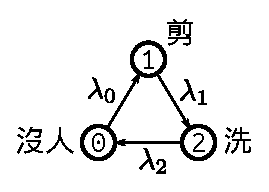
\includegraphics[scale=1.0]{hair_cut}
\end{center}
According to balance equation:
\begin{align*}
\lambda_0 \pi_0 & = \lambda_2 \pi_2 \\
\lambda_1 \pi_1 & = \lambda_0 \pi_0 \\
\lambda_2 \pi_2 & = \lambda_1 \pi_1
\end{align*}
And by $\pi_0 + \pi_1 + \pi_2 = 1$, we can represent $\pi_0$, $\pi_1$, $\pi_2$ by $\lambda_0$, $\lambda_1$, and $\lambda_2$.
\end{frame}

\begin{frame}{Example: Birth and death process}
According to balance equation:
\begin{align*}
\beta_0 \pi_0 & = \delta_1 \pi_1 \\
(\beta_1 + \delta_1)\pi_1 & = \beta_0 \pi_0 + \delta_2 \pi_2 \\
& \vdots \\
(\beta_n + \delta_n)\pi_n & = \beta_{n-1} \pi_{n-1} + \delta_{n+1} \pi_{n+1}
\end{align*}
which implies
\begin{align*}
\beta_0 \pi_0 & = \delta_1 \pi_1 \\
\beta_1 \pi_1 & = \delta_2 \pi_2 \\
& \vdots \\
\beta_n \pi_n & = \delta_{n+1} \pi_{n+1}
\end{align*}
\end{frame}

\begin{frame}{Example: Birth and death process (cont.)}
\begin{align*}
\pi_1 & = \frac{\beta_0}{\delta_1} \pi_0 \\
\pi_2 & = \frac{\beta_1}{\delta_2} \pi_1 = \frac{\beta_1 \beta_0}{\delta_2 \delta_1}\pi_0 \\
& \vdots \\
\pi_n & = \frac{\beta_0 \beta_1 \cdots \beta_{n-1}}{\delta_1 \delta_2 \cdots \delta_n} \pi_0
\end{align*}
By $\sum_{i\geq 0} \pi_i = 1$, we have
\[
\pi_0 = \frac{1}{1 + \sum_{k\geq 1}\frac{\beta_0 \beta_1 \cdots \beta_{k-1}}{\delta_1 \delta_2 \cdots \delta_k}}
~\text{and}~ \pi_n = \frac{\beta_0 \beta_1 \cdots \beta_{n-1}}{\delta_1 \delta_2 \cdots \delta_n
(1 + \sum_{k\geq 1}\frac{\beta_0 \beta_1 \cdots \beta_{k-1}}{\delta_1 \delta_2 \cdots \delta_k})}
\]
\end{frame}

\begin{frame}{Example: Birth and death process (cont.)}
As a matter of fact,
\[
\sum_{k\geq 1}\frac{\beta_0 \beta_1 \cdots \beta_{k-1}}{\delta_1 \delta_2 \cdots \delta_k} < \infty
\iff
\sum_{i\geq 0} \pi_i = 1
\]
Ohterwise, each $\pi_i$ would have value $0$.
\end{frame}

\begin{frame}{Example: M/M/s servers}
\[
\beta_n = \beta, \qquad \delta_n = \left\{
\begin{array}{l l}
n\cdot \delta & \quad\text{if } n < s \\
s\cdot \delta & \quad\text{if } n\geq s \\
\end{array}
\right.
\]
To make $\sum_{i\geq 0} \pi_n = 1$,
\begin{align*}
\sum_{k\geq 1}\frac{\beta_0 \beta_1 \cdots \beta_{k-1}}{\delta_1 \delta_2 \cdots \delta_k} < \infty
& \iff
\sum_{k\geq s}\frac{\beta^k}{(s\cdot \delta)^k} < \infty \\
& \iff 
\frac{\beta}{s\cdot \delta} < 1
\iff
\frac{\beta}{\delta} < s
\end{align*}
\end{frame}

\begin{frame}{Example: Server crash}
There are $s$ servers.
Each server has parameter $\beta$ of crashing.
Only one person is fixing the servers, with parameter $\delta$.
We want to know:
\begin{enumerate}
\item The time proportion that no server is in crash.
\item Expectation number of crashing servers.
\end{enumerate}
\vspace{\baselineskip}
\textbf{Solution}:\\
Let state $n$ represents that there are $n$ crashed servers.
\[
\delta_n = \left\{ 
\begin{array}{l l}
\delta & \quad\forall 1\leq n\leq s \\
0 & \quad\text{otherwise}
\end{array}
\right.
\qquad
\beta_n = \left\{
\begin{array}{l l}
(s - n)\beta & \quad\forall 0\leq n\leq s \\
0 & \quad\text{otherwise}
\end{array}
\right.
\]
\end{frame}

\begin{frame}{Solution to question 1}
\begin{align*}
\pi_0 & = \frac{1}{1 + \sum_{k=1}^s \frac{\beta_0 \beta_1 \cdots \beta_{k-1}}{\delta_1 \delta_2 \cdots \delta_k}} \\
& = \frac{1}{1 + \sum_{k=1}^s \frac{s\beta\cdot (s-1)\beta \cdots (s-k+1)\beta}{\delta^k}} \\
& = \frac{1}{1 + \sum_{k=1}^s \left( \frac{\beta}{\delta} \right)^k \frac{s!}{(s-k)!}}
\end{align*}
\end{frame}

\begin{frame}{Solution to question 2}
From previous page, we know
\[
\pi_n = \frac{\left( \frac{\beta}{\delta} \right)^n \frac{s!}{(s-n)!}}
{1 + \sum_{k=1}^s \left( \frac{\beta}{\delta} \right)^k \frac{s!}{(s-k)!}}
\]
Hence, the expectation is
\[
\sum_{n=0}^s n\cdot \pi_n
\]
\end{frame}

\begin{frame}{Example: Server crash advanced}
Given $n$ servers.
The working time parameter for the $i$th server is $s_i$.
And the fixing time parameter is $r_i$.
There's only one TA, who will fix the most recently crashed server in the first priority.\\
\vspace{\baselineskip}
We use $(i_1, i_2, \ldots, i_k)$ to represent the state that $k$ servers crash, $i_j$ is the $j$th recently crashed server.
And use $\phi$ as the state that all the servers are working.
Hence, we have $\sum_{k=0}^n \binom{n}{k} k!$ different states.
\end{frame}

\begin{frame}{Example: Server crash advanced (cont.)}
According to balance equation:
\[
\sum_{i=1}^n s_i\cdot \pi(\phi) = \sum_{i=1}^n r_i\cdot \pi(i)
\]
\begin{align*}
& \left( r_{i_1} + \sum_{i\notin\{i_1, i_2, \ldots, i_k\}}s_i \right)\cdot \pi(i_1, i_2, \ldots, i_k) \\
= &~ s_{i_1}\cdot \pi(i_2, \ldots, i_k) + \sum_{i\notin\{i_1, i_2, \ldots, i_k\}} r_i\cdot \pi(i, i_1, i_2, \ldots, i_k)
\end{align*}
\end{frame}

\begin{frame}{Example: Server crash advanced (cont.)}
\begin{align*}
\pi(\phi) & = \frac{1}{1 + \sum_{(i_1, i_2, \ldots, i_k)} \frac{s_{i_1} s_{i_2}\cdots s_{i_k}}{r_{i_1} r_{i_2}\cdots r_{i_k}}} \\
\pi(i_1, i_2, \ldots, i_k) & = \frac{s_{i_1} s_{i_2}\cdots s_{i_k}}{r_{i_1} r_{i_2}\cdots r_{i_k}}\cdot \pi(\phi)
\end{align*}
\end{frame}

\begin{frame}{Time reversibility}
\begin{itemize}
\item Assume $\mathbb{X}$ is irreducible and positive recurrent.
We say $\mathbb{X} \to \mathbb{X}^*$ is a discretization that changes each inter-arrival time of $\mathbb{X}$ to $1$.
\item $\mathbb{X}^*$ can now be seen as a discrete Markov chain, which still satisfies irreducible and positive recurrent.
\item Assume $\mathbb{X}^*$ is aperiodic, we can take the matrix $\mathbb{P}$ of $\mathbb{X}$ as the transition matrix of $\mathbb{X}^*$ in the discrete Markov chain.
\item We know that $\mathbb{X}^*$ has the limiting probability vector $\pi^*$, and
\[
\pi^*\times \mathbb{P} = \pi^*, \quad \sum_{i\in S} \pi_i^* = 1
\]
\end{itemize}
\end{frame}

\begin{frame}{Time reversibility (cont.)}
According to balance equation,
\[
\lambda_j\cdot \pi_j = \sum_{k\in S} \lambda_k\cdot \pi_k\cdot \mathbb{P}[k,j]
\]
If we let $\hat{\pi} = (\lambda_1 \pi_1, \lambda_2 \pi_2, \ldots)$, we know that
$\hat{\pi}\times \mathbb{P} = \hat{\pi}$ and $\frac{\hat{\pi}}{\sum_{i\in S} \hat{\pi}_i}$ is the unique vector that is $\pi^*$. Hence,
\[
\pi_i^* = \frac{\pi_i\cdot \lambda_i}{\sum_{j\in S} \pi_j\cdot \lambda_j} ~\text{and}~
\pi_i = \frac{\pi_i^* / \lambda_i}{\sum_{j\in S} \pi_j^* / \lambda_j}
\]
\end{frame}

\begin{frame}{Time reversibility (cont.)}
According to the time reversibility of discrete Markov chain, we know
\begin{itemize}
\item The reversed chain $\mathbb{Y}^*$ of $\mathbb{X}^*$, which is also a Markov chain, has transition matrix $\mathbb{Q}$ such that
\[
\pi_i^*\cdot \mathbb{Q}[i,j] = \pi_j^*\cdot \mathbb{P}[j,i] \quad\forall i,j \in S
\]
\item If
\[
\pi_i^*\cdot \mathbb{P}[i,j] = \pi_j^*\cdot \mathbb{P}[j,i] \quad\forall i,j \in S
\]
then $\mathbb{X}^*$ is time-reversible.
\item If we can find any vector $\hat{\pi}$ such that
\[
\hat{\pi}_i\cdot \mathbb{P}[i,j] = \hat{\pi}_j\cdot \mathbb{P}[j,i] \quad\forall i,j \in S ~\text{and}~
\sum_{i\in S} \hat{\pi}_i = 1
\]
then $\hat{\pi} = \pi^*$.
\end{itemize}
\end{frame}

\begin{frame}{Time reversibility (cont.)}
\begin{itemize}
\item If $\mathbb{X}$ is in steady state, which means that $P(X(t) = i) = \pi_i ~\forall i\in S$, we can prove that the reversed chain $\mathbb{Y}$ of $\mathbb{X}$ is also a continuous Markov chain.
\item Since the discretization of $\mathbb{Y}$ is $\mathbb{Y}^*$, $\mathbb{Q}$ would also be the matrix for $\mathbb{Y}$.
\item To characterize $\mathbb{Y}$, we use $\mathbb{Q}[i,j] = \pi_j^*\cdot \mathbb{P}[j,i] / \pi_i^*$ and each $\lambda_i$ are the same as $\mathbb{X}$.
\end{itemize}
\end{frame}

\begin{frame}{Time reversibility (cont.)}
If $\mathbb{X}$ is time reversible, then $\mathbb{Q} = \mathbb{P}$, which means that $\mathbb{X}^*$ is also time reversible.
And we know that
\begin{align*}
& \pi_i^*\cdot \mathbb{P}[i,j] = \pi_j^*\cdot \mathbb{P}[j,i] \\
\iff & \lambda_i\cdot \pi_i\cdot \mathbb{P}[i,j] = \lambda_j\cdot \pi_j\cdot \mathbb{P}[j,i] \\
\iff & \pi_i\cdot q_{ij} = \pi_j\cdot q_{ji}
\end{align*}
\begin{itemize}
\item LHS is the Poisson rate of $i\to j$ transitions.
\item RHS is the Poisson rate of $j\to i$ transitions.
\end{itemize}
\end{frame}

\begin{frame}{Example: Birth and death process}
Since $\pi_i\cdot q_{i,(i+1)}$ is the Poisson rate (i.e. $\lambda$) of $i\to i+1$ transitions,
\[
E[\text{number of $i\to i+1$ in $[s,s+t]$}] = \pi_i\cdot q_{i,(i+1)}\cdot t
\]
Hence
\begin{align*}
\pi_i\cdot q_{i,(i+1)} & = \frac{E[\text{number of $i\to i+1$ in $[s,s+t]$}]}{t} \\
& \colorbox{yellow}{=} \frac{E[\text{number of $i + 1\to i$ in $[s,s+t]$}]}{t} = \pi_{i+1}\cdot q_{(i+1),i}
\end{align*}
\begin{itemize}
\item Then we know that B \& D process is time reversible.
\item \colorbox{yellow}{=} is because one must go back from $i+1$ to $i$ to go from $i$ to $i+1$ again.
\end{itemize}
\end{frame}

\begin{frame}{Example: M/M/s servers}
M/M/s is a birth and death process, it's time-reversible when in steady state ($\frac{\beta}{\delta} < s$).
We want to prove that the overall process of job departing is a Poisson process with rate $\beta$.\\
\vspace{\baselineskip}
\textbf{Proof}: Since it's time reversible, the rate of $i\to i-1$ is equal to the rate of $i-1\to i$, which is $\beta$.
\end{frame}

\begin{frame}{Example: M/M/1 server}
In the M/M/1 system, if a job $J$ stays for a time interval $t$, what is the distribution of the number of jobs already in the system when $J$ enter this system?\\
\vspace{\baselineskip}
\textbf{Solution}: Assume $J$ arrives at $s$ and depart at $s+t$, we know that all the jobs queuing in system at time $s$ will depart in $[s,s+t]$, and the distribution of job departing in $[s,s+t]$ is Poisson with parameter $\beta\cdot t$ from the previous example.
\end{frame}

\begin{frame}{Theorem on the other direction}
\begin{theorem}
If there exists a nonnegative vector $\pi$ with 
\[
\sum_{i\in S} \pi_i = 1 ~\text{and}~ \pi_i\cdot q_{ij} = \pi_j\cdot q_{ji}\quad\forall i,j\in S
\]
then $\mathbb{X}$ is a time-reversible chain and $\pi$ is the limiting probability of $\mathbb{X}$.
\end{theorem}
\end{frame}

\begin{frame}{Example: Server crash advanced}
Given $n$ servers. The working time parameter for the $i$th server is $\beta_i$.
And the fixing time parameter is $\delta_i / k$ if there are $k$ servers currently crashed.
We want to know if this process is time reversible?\\
\vspace{\baselineskip}
We use a set $D\subseteq \{1,2,\ldots,n\}$ to represent the state of crashed servers.
There are $2^n$ different states.
If $i\notin D$ and $|D| = k-1$ with $k\geq 1$, then
\[
q_{D,D\cup\{i\}} = \beta_i ~\text{and}~ q_{D\cup\{i\},D} = \frac{\delta_i}{k}
\]
\end{frame}

\begin{frame}{Example: Server crash advanced (cont.)}
We prove the time reversibility by guessing a $\pi$ to satisfy
\[
\pi_D\cdot \beta_i = \pi_{D\cup\{i\}}\cdot \frac{\delta_i}{k}
\]
that is
\begin{align*}
\pi_\phi & = \frac{1}{1 + \sum_{\phi\neq D\subseteq \{1,2,\ldots,n\}} |D|!\cdot \prod_{i\in D}\frac{\beta_i}{\delta_i}} \\
\pi_D & = (|D|!\cdot \prod_{i\in D}\frac{\beta_i}{\delta_i})\cdot \pi_\phi
\end{align*}
\end{frame}

\begin{frame}{Truncated Markov chain}
\begin{definition}
Given a set $A$ of states of $\mathbb{X}$, $\mathbb{X}^A$ is the \emph{truncated chain} of $\mathbb{X}$ w.r.t.\ $A$,
where the matrix of $q_{ij}$ is induced by $i,j\in A$.
\end{definition}
\begin{itemize}
\item We can see that if $\mathbb{X}$ is time reversible, so is $\mathbb{X}^A$.
Since we can find a $\pi^A$ that $\pi_i^A = \pi_i / \sum_{k\in A}\pi_k$.
\end{itemize}
\end{frame}

\begin{frame}{Uniformization}
\begin{definition}
\emph{Uniformization} is a transformation that makes $\mathbb{X}$ into $\mathbb{Y}_\lambda$, where $\lambda_i = \lambda\quad\forall i\in S$.
\end{definition}
\begin{itemize}
\item All the transitions of $\mathbb{Y}_\lambda$ forms a Poisson process with rate $\lambda$.
\end{itemize}
\end{frame}

\begin{frame}{Theorem: Transition matrix of uniformized chain}
\begin{theorem}
If $\mathbb{Q}$ is the transition matrix of $\mathbb{Y}_\lambda$, then
\[
Q_{ij}(t) = \sum_{n=0}^\infty \mathbb{Q}^n[i,j]\cdot e^{-\lambda t}\cdot \frac{(\lambda t)^n}{n!}
\]
\end{theorem}
\begin{itemize}
\item $Q_{ij}(t)$ is the transition probability function.
\item Note that $\mathbb{Q}^n[i,j]\neq (\mathbb{Q}[i,j])^n$.
\end{itemize}
\end{frame}

\begin{frame}{Proof}
Let $N(t)$ represents the number of transitions in $[0,t]$.
\begin{align*}
\text{LHS} & = \sum_{n=0}^\infty P(Y_\lambda(t)=j | Y_\lambda(0)=i, N(t)=n)
\cdot P(N(t)=n | Y_\lambda(0)=i) \\
& = \sum_{n=0}^\infty \mathbb{Q}^n[i,j]\cdot \frac{(\lambda t)^n e^{-\lambda t}}{n!} \\
& = \text{RHS}
\end{align*}
\end{frame}

\begin{frame}{Application of uniformization}
\begin{itemize}
\item Let $\mathbb{X}$ be a continuous Markov chain with $\lambda_i\leq \lambda\quad\forall i$.
\item We can think as the transition rate for all states $i$ are $\lambda$, but when the transition happens, it has probability $\lambda_i / \lambda$ that it will really transit to other state, and with probability $1 - (\lambda_i / \lambda)$ it will keep in state $i$.
\item We then have $\mathbb{Y}_\lambda$ with
\[
\mathbb{Q}[i,j] = \left\{
\begin{array}{l l}
1 - \frac{\lambda_i}{\lambda} & \quad i=j \\
\frac{\lambda_i}{\lambda}\cdot \mathbb{P}[i,j] & \quad i\neq j \\
\end{array}
\right.
\]
\end{itemize}
\end{frame}

\begin{frame}{Example}
For an example with only two states 0 and 1, where $\lambda_0 = \beta$ and $\lambda_1 = \delta$,
we do the uniformization with $\lambda = \beta + \delta$.
Then
\[
\mathbb{Q} = \begin{pmatrix}
\frac{\delta}{\beta + \delta} & \frac{\beta}{\beta + \delta} \\
\frac{\delta}{\beta + \delta} & \frac{\beta}{\beta + \delta} \\
\end{pmatrix}
\]
We can observe that $\mathbb{Q}^n = \mathbb{Q} \quad\forall n\geq 1$.
And we can obtain the value of each $Q_{ij}(t)$.
\end{frame}

\end{document}